\documentclass{article}

\usepackage{amssymb}
\usepackage{amsmath}
\usepackage{amsthm}
\usepackage{graphicx}
\usepackage{a4wide}
\usepackage[ruled,vlined]{algorithm2e}
\usepackage{color}
%\usepackage{hyperref}

\newtheorem{definition}{Definition}
\newtheorem{observation}{Observation}
\newtheorem{lemma}{Lemma}
\newtheorem{corollary}{Corollary}
\newtheorem{theorem}{Theorem}

\newtheorem*{example}{Example}

\newcommand{\Problem}[1]{\par\vspace{3mm}\noindent{\bf Problem{\hspace{1mm}}#1}\hspace{1mm}}
\newcommand{\Solution}{\par\vspace{3mm}\noindent{\bf Solution}\hspace{1mm}}

\newcommand{\NP}{\mathbf{NP}} %{\complsuperclassfont{NP}}
\renewcommand{\P}{\mathbf{P}} %{\complsuperclassfont{P}}

\newcommand{\Hide}[1]{}

\newcommand{\ignore}[1]{}


\newcommand{\setR}{\mathbb{R}}
\newcommand{\setN}{\mathbb{N}}
\newcommand{\mat}[1]{ \begin{pmatrix} #1 \end{pmatrix}}


\begin{document}

\title{Discrete Optimization}
\maketitle

\tableofcontents
\newpage

\vfill
\subsection*{Remarks}
The following scribe notes were developed during the summer term 2011
in parallel to a lecture given by Nikola Milosavljevic and Stefan Funke.
Some modifications and additions were made during the winter term 2012/3 when the
same lecture was held again by Stefan Funke and partly Martin Seybold. Further
changes during the winter term 2013/4. 
The scribe notes do not necessarily reflect everything that was covered in class
but should rather be seen as additional source to your own write-up.

\textcolor{blue}{\emph{Knowledge of Bellmann-Ford- and Dijkstra-Algorithm is of need.}}


\newpage

\section{Network Flow}
\subsection{MaxFlow}
Given a directed graph $G(V,E)$ with distinguished nodes $s\in V$ (source) and $t$ (sink), a capacity function $c:E\rightarrow \mathbb{R}^+$ \textcolor{blue}{\emph{($c:E\rightarrow \mathbb{Z}^+_0$)}} we are interested in determining a maximum \emph{flow} from $s$ to $t$, that is, a function $f:E\rightarrow \mathbb{R}^+$ \textcolor{blue}{\emph{($f:E\rightarrow \mathbb{Z}^+_0$)}} assigning each edge a
non-negative flow value such that:
\begin{itemize}
\item $\displaystyle \sum_{e=(v,.)} f(e)=\sum_{e=(.,v)} f(e)$ for all $v\in V-\{s,t\}$, that is, the inflow equals the outflow for any node $v$ which is different from source or sink ({\bf flow conservation constraint})
\item $f(e)\leq c(e)$ for all $e\in E$, that is the flow on an edge never exceeds the capacity of the edge ({\bf capacity constraint})
\end{itemize}


Goal is to maximize the value of the flow, that is, the outflow $\sum_{e=(s,.}f(e)$ from $s$ which happens to be equivalent to the inflow $\sum_{e=(.,t)} f(e)$ into $t$ (no unit of flow can get lost or be added at any other node due to the flow conservation constraints).

\begin{figure}
\begin{center}
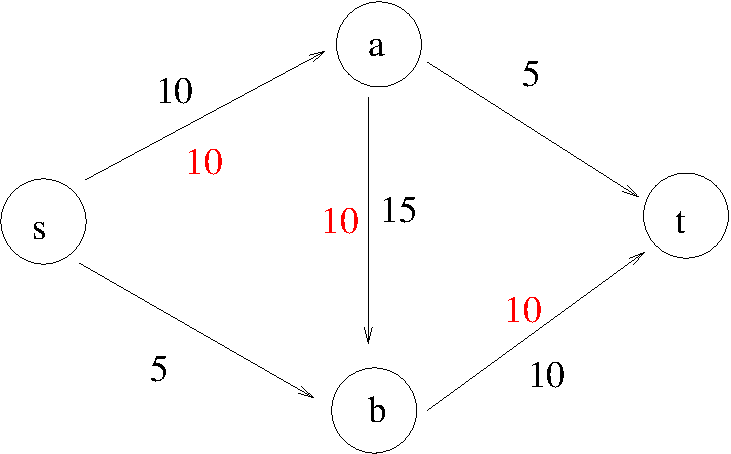
\includegraphics[width=6cm]{Figs/flow1.pdf} 
\hspace{1cm}
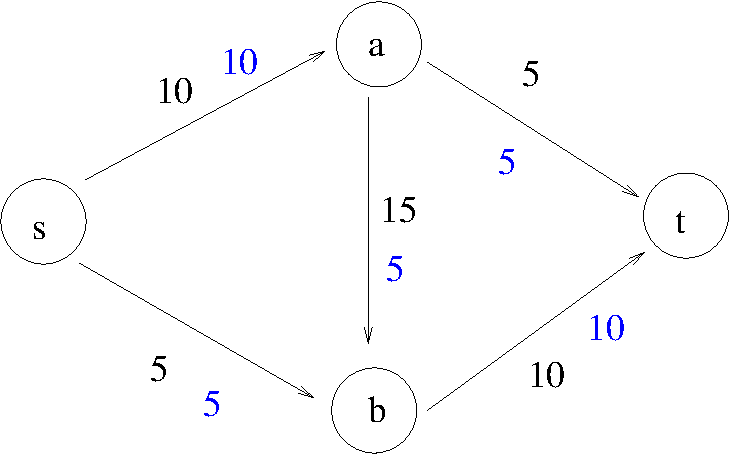
\includegraphics[width=6cm]{Figs/flow1b.pdf}
\end{center}
\caption{Left: Sample Flow (red) of value $10$ for a small network. Capacities are given in black. Right: Better Flow (blue) of value $15$.}\label{fig:flow1}
\end{figure}

Consider Figure \ref{fig:flow1},left, for an example of a valid flow (in red) for given edge capacities (in black). The value of this flow is $10$, no edge capacity is violated and at all nodes except for source and sink, the inflow equals the outflow.

\textcolor{blue}{\emph{Optimal flow in example is easily derivable by looking at it, but whats the corresponding algorithm?}}

How could we compute such a flow? A first attempt at an algorithm could be as follows:
\begin{verbatim}
   1. start with a zero-flow
   2. find a path consisting of edges with non-zero remaining capacities from s to t;
      send as much flow as possible across this path 
   3. repeat 2. as long as possible
\end{verbatim}
In step 2, the maximum amount of flow to be sent across a path is determined by its bottleneck -- the edge with smallest capacity along the path.
In fact, our algorithm might compute the flow depicted in Figure \ref{fig:flow1}, left, if the first path found was $s\rightarrow a\rightarrow b\rightarrow t$; then no further path of non-zero remaining capacities from $s$ to $t$ exists and the algorithm terminates. One important question remains open, though: Is the resulting flow optimal?

Unfortunately it turns out that it is not optimal. In Figure \ref{fig:flow1}, right, we see a flow (in blue) of value $15$, which could be the result of our algorithm (if the e.g. first the path $s\rightarrow a\rightarrow t$ followed by $s\rightarrow b \rightarrow t$ and $s\rightarrow a \rightarrow b \rightarrow t$ was picked) which could not be constructed from the flow on the left. So we better think of a refined algorithm.

The crucial observation that leads to an algorithm which actually computes a maximum flow can  be explained in Figure \ref{fig:flow1}, left. While there is no edge to send flow from $b$ to $a$, in presence of the red flow, there is still the possibility to send flow from $b$ to $a$ by \emph{sending less flow} from $a$ to $b$. In fact this corresponds to a virtual edge from $b$ to $a$ with capacity $10$ (since with the red flow being present, we can send at most $10$ units of flow less from $a$ to $b$).

Based on this observation we define for a given network $G(V,E,c)$ and flow $f:E\rightarrow \mathbb{R}^+$ the so-called \emph{residual network} $G_f(V, E_f, c_f)$ as follows:
\begin{itemize}
\item for any edge $e\in E$ with $c(e)>f(e)$ we have $e\in E_f$ with $c_f(e)=c)(e)-f(e)$
\item for any edge $e=(v,w)\in E$ with $f(e)>0$ we have an edge $e_R=(w,v)\in E_f$ with $c_f(e_R)=f(e)$
\end{itemize}
The first rule creates edges with non-zero remaining capacity in $G_f$, the second introduces all the virtual reverse edges for edges across which actual flow is sent. See Figure 6 for a flow in $G$ and the resulting residual network.
\begin{figure}
\begin{center}
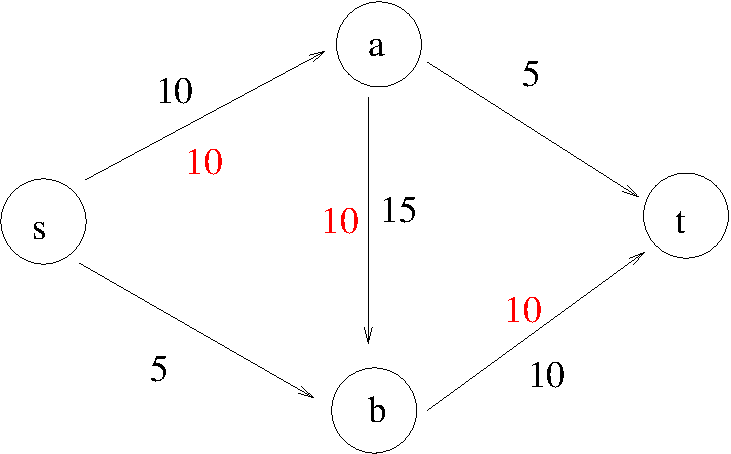
\includegraphics[width=6cm]{Figs/flow1.pdf} 
\hspace{1cm}
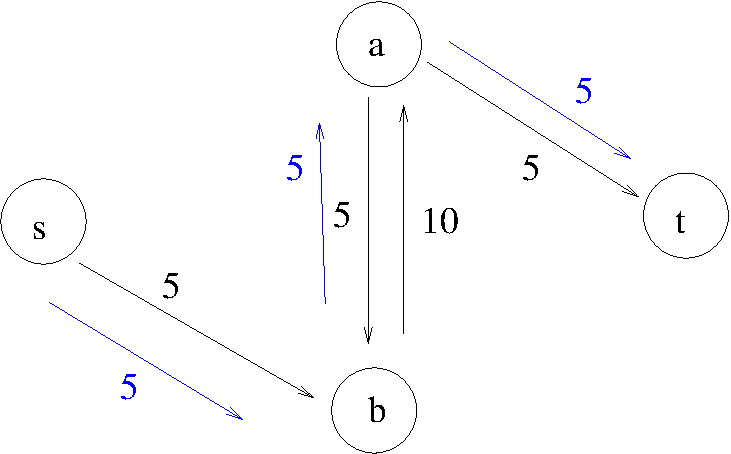
\includegraphics[width=6cm]{Figs/flowRN1.pdf}

\vspace{1cm}
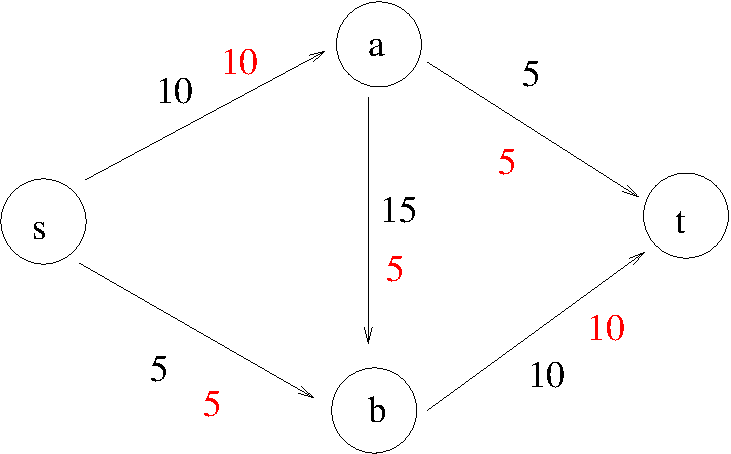
\includegraphics[width=6cm]{Figs/flowRN2.pdf}
\hspace{1cm}
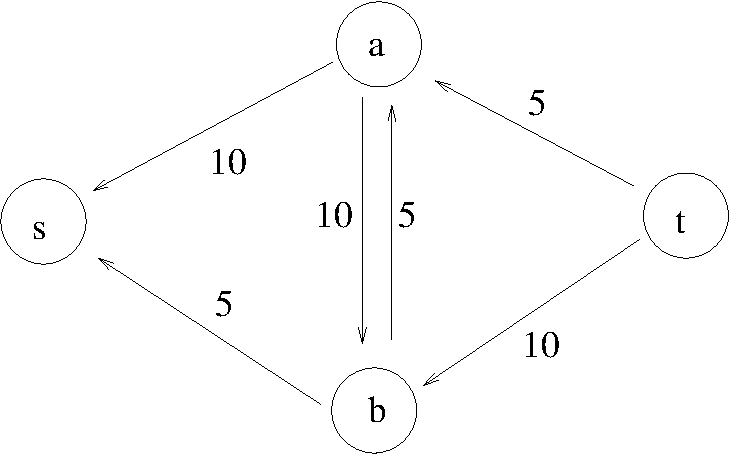
\includegraphics[width=6cm]{Figs/flowRN3.pdf}
\end{center}
\caption{Sample Flow (red) for a small network (upper left). Resulting residual network with possible augmenting path(upper right). Resulting total flow (lower left). Last residual network without $s$-$t$ path.}\label{fig:flowRN}
\end{figure}

Extending our first attempt at an algorithm in a natural way is then to search for $s$-$t$ paths in this residual network, sending flow across such a path (the amount of which is determined by the \emph{bottleneck} of the path, that is, its minimum capacity edge) if such exists, rebuilding the residual network etc. until no further path in the residual network exists. In fact this is the algorithm which we will be using and proving correctness for, it is called the \emph{Ford-Fulkerson} algorithm (google it!).	

\begin{verbatim}
   FORD-FULKERSON
   1. start with the zero-flow f=0
   2. Construct the residual network G_f
   3. find a path consisting of edges with non-zero remaining capacities from s to t in G_f;
      send as muchflow as possible across this path; add this flow to f
      if no such path exists, stop the algorithm and return f
   4. goto 2.
\end{verbatim}

It is not hard to see that this algorithm (like the previous, incorrect one) terminates:

\begin{lemma}
The algorithm terminates in $\min\left(\sum_{e=(s,.)} c(e), \sum_{e=(.,t)} c(e)\right)$ steps.
\end{lemma}
\begin{proof}
In each round of the algorithm the net flow from $s$ to $t$ increases by at least $1$, hence
the total number of rounds is upper bounded by the sum of the outgoing capacities of $s$ and
the incoming capacities of $t$.
\end{proof}

For the new algorithm we can also prove that it computes indeed the maximum possible flow from $s$ to $t$.
To that end we first need a simple observation to derive upper bounds.

\begin{definition}
Let $G(V,E)$ be a directed graph, $A\subset V$  be a subset of the nodes.
The \emph{directed cut} induced by $A$ is defined as $\mbox{dcut}(A):=\{e=(v,w): v\in A, w\notin A\}$, that is,
the set of edges which have their source in $A$ and their target not in $A$.
\end{definition}

It is not hard to see that any such directed cut induces an upper bound on the maximum flow from $s$ to $6$
\begin{lemma}
For a directed graph $G(V,E)$ with edge capacities $c:E\rightarrow \mathbb{R}^+$ let $A\subset V$ be a subset of the nodes with $s\in A$, $t\notin A$, then $\sum_{e\in\mbox{dcut}(A)} c(e)$ is an upper bound on the max flow from $s$ to $t$.
\end{lemma}
\begin{proof}
Consider a maximum flow from $s$ to $t$; any unit of this flow has to cross the boundary from $A$ to $V-A$ somewhere. The amount of flow that can cross this boundary is bounded by the above quantity.
\end{proof}

The idea of our correctness proof is to consider the residual network of the final flow that our algorithm has produced and use this to exhibit a set $A$ inducing a directed cut which realizes an upper bound matching the flow our algorithm has produced.

To that end consider the set $A^*$ which consists of all nodes that are reachable from $s$ in the residual network $G_f$ of the flow $f$ that our algorithm has computed and consider the edges leaving and entering $A^*$.
\begin{lemma}
Let $f$ be the flow produced by our algorithm for a network $G(V,E)$ with edge capacities $c:E\rightarrow \mathbb{R}^+$, $e=(v,w)\in E$ with $\{v,w\}\cap A^*=1$. Then we have:
\begin{itemize}
\item if $v\in A^*$, that is, we have an edge $(v,w)$ out of  $A^*$, then $f(e)=c(e)$
\item if $w\in A^*$, that is, we have an edge $(v,w)$ into $A^*$, then $f(e)=0$ 
\end{itemize}
\end{lemma}
\begin{proof}
For the first part, observe that if $f(e)>0$, then there is an edge from $v$ to $w$ in the residual network of positive capacity making $w$ reachable from $s$ in $G_f$, contradicting the fact that $w\notin A^*$.
For the second part, note that if $f(e)>0$, then there is a back edge $(w,v)$ out of $A^*$ in $G_f$ with positive capacity, making $v$ reachable from $s$, also contradicting non-membership of $v$ in $A^*$.
\end{proof}

This almost concludes the correctness proof for the Ford-Fulkerson algorithm. Due to the previous Lemma we know that the value of the flow $f$ produced is $\displaystyle \sum_{e=(v,w): v\in A^*, w\notin A^*} f(e)=\sum_{e=(v,w): v\in A^*, w\notin A^*} c(e)$, but as the directed cut induced by $A^*$ implies an upper bound of\\ $\displaystyle\sum_{e=(v,w): v\in A^*, w\notin A^*} f(e)$, the two bounds match and we have shown optimality of $f$.

\begin{corollary}
The Ford-Fulkerson algorithm terminates and computes a maximum flow.
\end{corollary}

Note that the running time of Ford-Fulkerson in this version can only be bounded by $O(C(n+m))$ where $C$ denotes the sum of capacities. $O(m+n)$ time is required for each construction of the residual network and construction of an augmenting path. Unfortunately $C$ might not be polynomial in the input size. See Figure \ref{FIG:FFbad} for an example where FF might take a very long time (for a bad sequence of augmenting paths).
\begin{figure}
\centering
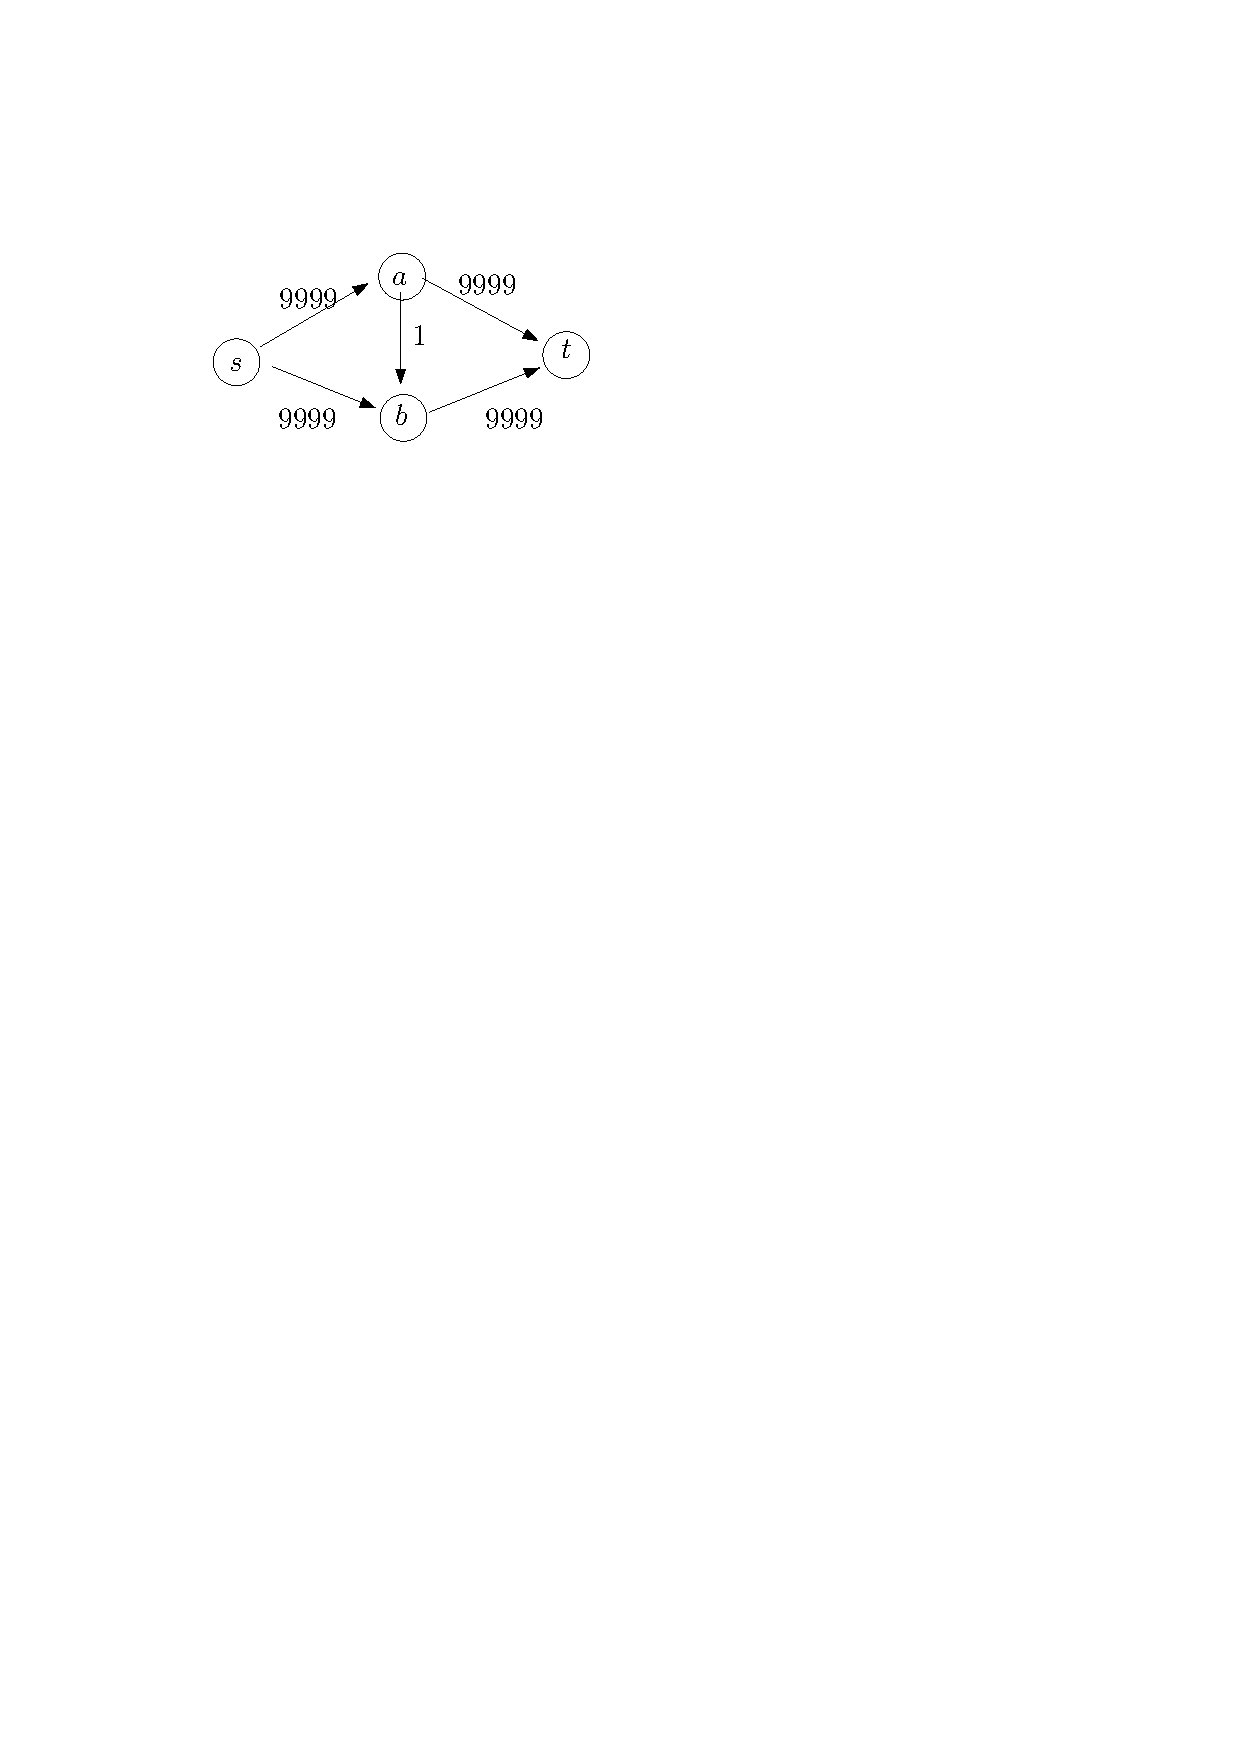
\includegraphics[width=6cm]{Figs/FF-bad.pdf}
\caption{Example where FF might take a long time.}\label{FIG:FFbad}
\end{figure}


\subsubsection{Capacity Scaling}
In the following we will describe a modification of the original FF algorithm that allows to prove a polynomial running time. The idea is first to search for augmenting paths with large bottlenecks only, and only if such paths cannot be found anymore, search for augmenting paths with smaller bottlenecks. The algorithm can be described as follows:
\begin{verbatim}
	start with a zero-flow f
	D= next smaller power of two of max capacity
	while (D>=1) do
	   Gf=residual network of G wrt f restricted to edges of capacity >=D
	   while there is an augmenting path in Gf do
	      augment f, recompute Gf
	   done
	   D=D/2
	done
\end{verbatim}

Observe that the algorithm certainly terminates and produces a maximum flow as each augmentation increases the flow by at least $1$ and when $D=1$, $G_f$ is the residual network as in the original Ford-Fulkerson algorithm.
Let us try to argue now that the number of augmentations is polynomially bounded.
Note that the outer loop is executed $O(\log C)$ times where $C$ denotes the maximum capacity of an edge in the network.

\begin{lemma}
Let $f_D$ be the flow after completing augmentations with capacity value $D$. Then the maximum flow of the network is bounded by $val(f_D)+mD$.
\end{lemma}
\begin{proof}
Consider the residual network $G_{f_D}$ after the last augmentation with capacity value $D$ (including all edges with capacity less than $D$). Let $A$ be the set of nodes reachable from $s$ if all edges of capacity $<D$ are removed from $G_{f_D}$. $A$ induces a directed cut of some capacity $C$. If we subtract the current flow $f_D$ from the edge capacities of the edges leaving $A$, we know that all these edges have remaining capacity $<D$. There can be at most $m$ such edges, hence the $C-val(f_D)<mD$.
\end{proof}

\begin{lemma}
For fixed $D$, the inner while loop is executed at most $2m$ times.
\end{lemma}
\begin{proof}
Starting with a flow $f$ for fixed $D$, we know (from the previous round with $2D$ that the total flow is bounded by $val(f)+2Dm$. In each round of the inner while loop, the flow is increased by at least $D$, hence there can be at most $2m$ round of the inner while loop.
\end{proof}

\begin{theorem}
Ford-Fulkerson with capacity scaling terminates after $O(2m(m+n)\log C)=O(m^2\log C)$ steps.
\end{theorem}

\subsubsection{Shortest Augmenting Path (Edmonds-Karp Algorithm)}
Capacity scaling leads to a running time guarantee which still depends on the magnitude of the capacities.
In the following we will show that when augmenting always using a \emph{shortest} path (in terms of hop distance), the running time can be bounded by $O(m^2n)$.

So consider in the following the variant of Ford-Fulkerson, where we always augment on a \emph{shortest path} in the current residual network $G_f$. Such a shortest path can be computed using Breadth-First-Search in $O(m+n)$.

We will prove the following two lemmas 
\begin{lemma}\label{lem:SPnondec}
During the course of the algorithm, the length of the augmenting paths never decreases.
\end{lemma}
\begin{lemma}\label{lem:SPinc}
After at most $O(m)$ augmentations, the length of the augmenting path increases by at least one.
\end{lemma}

The two lemmas immediately lead to the following theorem:
\begin{theorem}
Ford-Fulkerson with shortest-path augmentation terminates after $O(m^2n)$ steps.
\end{theorem}

Let us prove the two lemmas in the following:
\begin{proof}(Lemma \ref{lem:SPnondec})
Let $l(v)$ be the distance of $v$ from $s$ in the residual network. $G_l$ the subgraph of residual network which only contains edges $(u,v)$ with $l(v)=l(u)+1$. A path $\pi$ in the residual network is a shortest path if it is a path in $G_l$. When augmenting along a path $\pi$, two things can happen along this path: (a) edges in the residual network disappear (as their capacity is fully used up) or (b) back edges are created which have not been present before. None of these modifications to the residual network can increase the level of any node, though. Therefore, the distance to any node -- in particular also to $t$ -- never decreases.
\end{proof}

\begin{proof}(Lemma \ref{lem:SPinc})
Let $E_k$ be the set of edges at the beginning of a phase when the distance between $s$ and $t$ is $k$. As soon as the shortest path from $s$ to $t$ uses an edge not in $E_k$ it has length larger $k$. Since with every augmentation, at least one edge (the bottleneck edge) is eliminated from $E_k$, after at most $m$ steps, the length of the shortest path from $s$ to $t$ must increase.
\end{proof}

\subsubsection{Non-integral Capacities}
So far we have always assumed \emph{integral} edge capacities, our termination and running time argumentation crucially relied on that. If edge capacities are real numbers, though, termination cannot be guaranteed and there are simple examples where Ford-Fulkerson not even converges towards the maximum flow (google it!).



\subsection{MinCostFlow}
\textcolor{blue}{\emph{MinCostFlow is a generalization of MaxFlow, as we can now model more than one source or sink.}}

Let us now consider an extension of the maxFlow problem where we also have to take into account \emph{costs}.
So we are given a directed network $G(V,E)$ with capacities $cap:E\rightarrow \mathbb{N}$ and costs $c:E\rightarrow \mathbb{Z}$. Furthermore, we have a function $b:V\rightarrow \mathbb{Z}$ which determines whether a node $v$ has a supply/surplus \textcolor{blue}{\emph{"`Ueberfluss"'}} of flow ($b(v)>0$) or a demand of flow ($b(v)<0)$; there might also be nodes which only act as relays ($b(v)=0$).

We assume that the surplus equals the demand, that is, $\displaystyle \sum_{v:b(v)<0} b(v)=-\sum_{v:b(v)>0} b(v)$.
The goal of the minCostFlow problem is to determine a flow $f:E\rightarrow \mathbb{N}$ such that
\begin{itemize}
\item $\forall e\in E: 0\leq f(e)\leq cap(e)$ (flow on an edge does not exceed the capacity \textcolor{blue}{\emph{capacity constraint}})
\item $\forall v\in V$: $\displaystyle b(v)+\sum_{e=(w,v)}f(e)=\sum_{e=(v,w)}f(e)$ (incoming and outgoing flow together with the surplus/deficit of the vertex balance out)
\item $\displaystyle\min \sum_{e\in E} f(e)c(e)$ (minimizing the total cost of the flow)
\end{itemize}

See Figure \ref{fig:minCostFlow-Ex1} for an example of a mcf instance as well as a feasible, but possibly not cost-optimal flow.

\begin{figure}
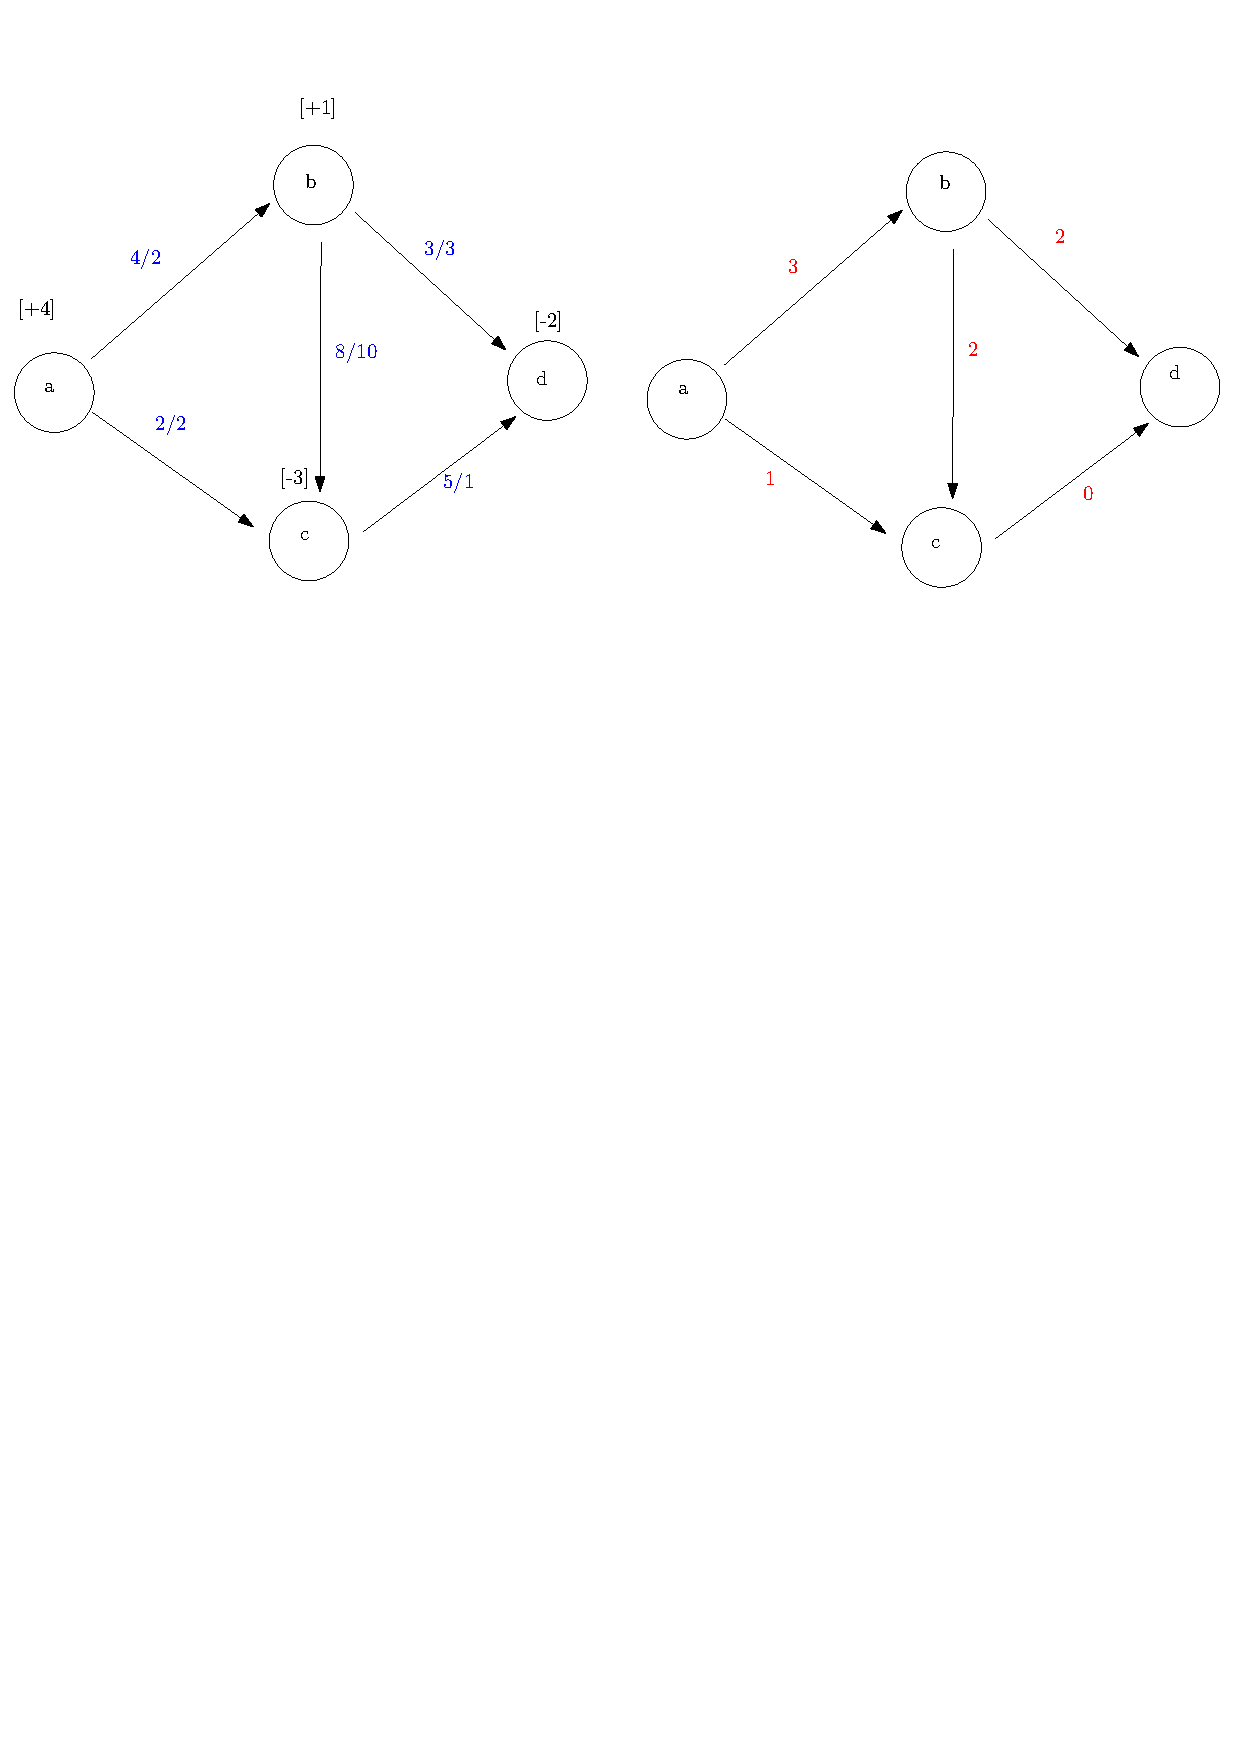
\includegraphics[width=\textwidth]{Figs/minCostFlow-Ex1.pdf}
\caption{MinCostFlow instance on the left; demand/surplus in brackets at the nodes, capacities/costs written at the edges. Feasible flow on the right (in red) of cost 34. \textcolor{blue}{\emph{(Left Value on edges is the capacity and the right value is the cost. The cost in the right image is calculated as follows $3*2+1*2+2*10+2*3 = 34$) }}}\label{fig:minCostFlow-Ex1} 
\end{figure}

\subsubsection{MinCostFlow via Cycle Cancelling}
Note that it is easy to obtain a \emph{feasible} flow via a single maxFlow computation: create a supersource $s$ which has an edge to each node $v\in V$ with $b(v)>0$ with capacity $b(v)$, and a supersink $t$ which has an incoming edge from each $w\in V$ with $b(w)<0$ with capacity $-b(w)$.
So let us assume that we have feasible flow and we want to decrease its cost.

\textcolor{blue}{\emph{Feasible flow in original network exists iff max flow ($f$ from $s$ to $t$) in this network has value $\sum_{v:b(v)>0} b(v)$}}

We proceed quite similar as for maxFlow in that we consider the \emph{residual network} $G'(V,E')$ for a given network $G(V,E)$ and a flow $f$. For each edge $e=(v,w)\in E$ with cost $c(e)$ and capacity $cap(e)$ we construct up to two edges $e_1, e_2$ in $G'$ as follows:
\begin{itemize}
\item if $f(e)<cap(e)$ there is an edge $e_1=(v,w)$ with cost $c'(e_1)=c(e)$ and capacity $cap'(e_1)=cap(e)-f(e)$
	(a forward edge with the remaining capacity)
\item if $f(e)>0$ there is an edge $e_2=(w,v)$ with cost $c'(e_1)=-c(e)$ and capacity $cap'(e_2)=f(e)$ (a backward edge with negative cost and capacity equal to the forward flow)
\end{itemize}

In Figure \ref{fig:minCostFlow-Ex1-residual}, left we see the respective residual network for the above problem instance (Figure \ref{fig:minCostFlow-Ex1}) and flow. 

\begin{figure}
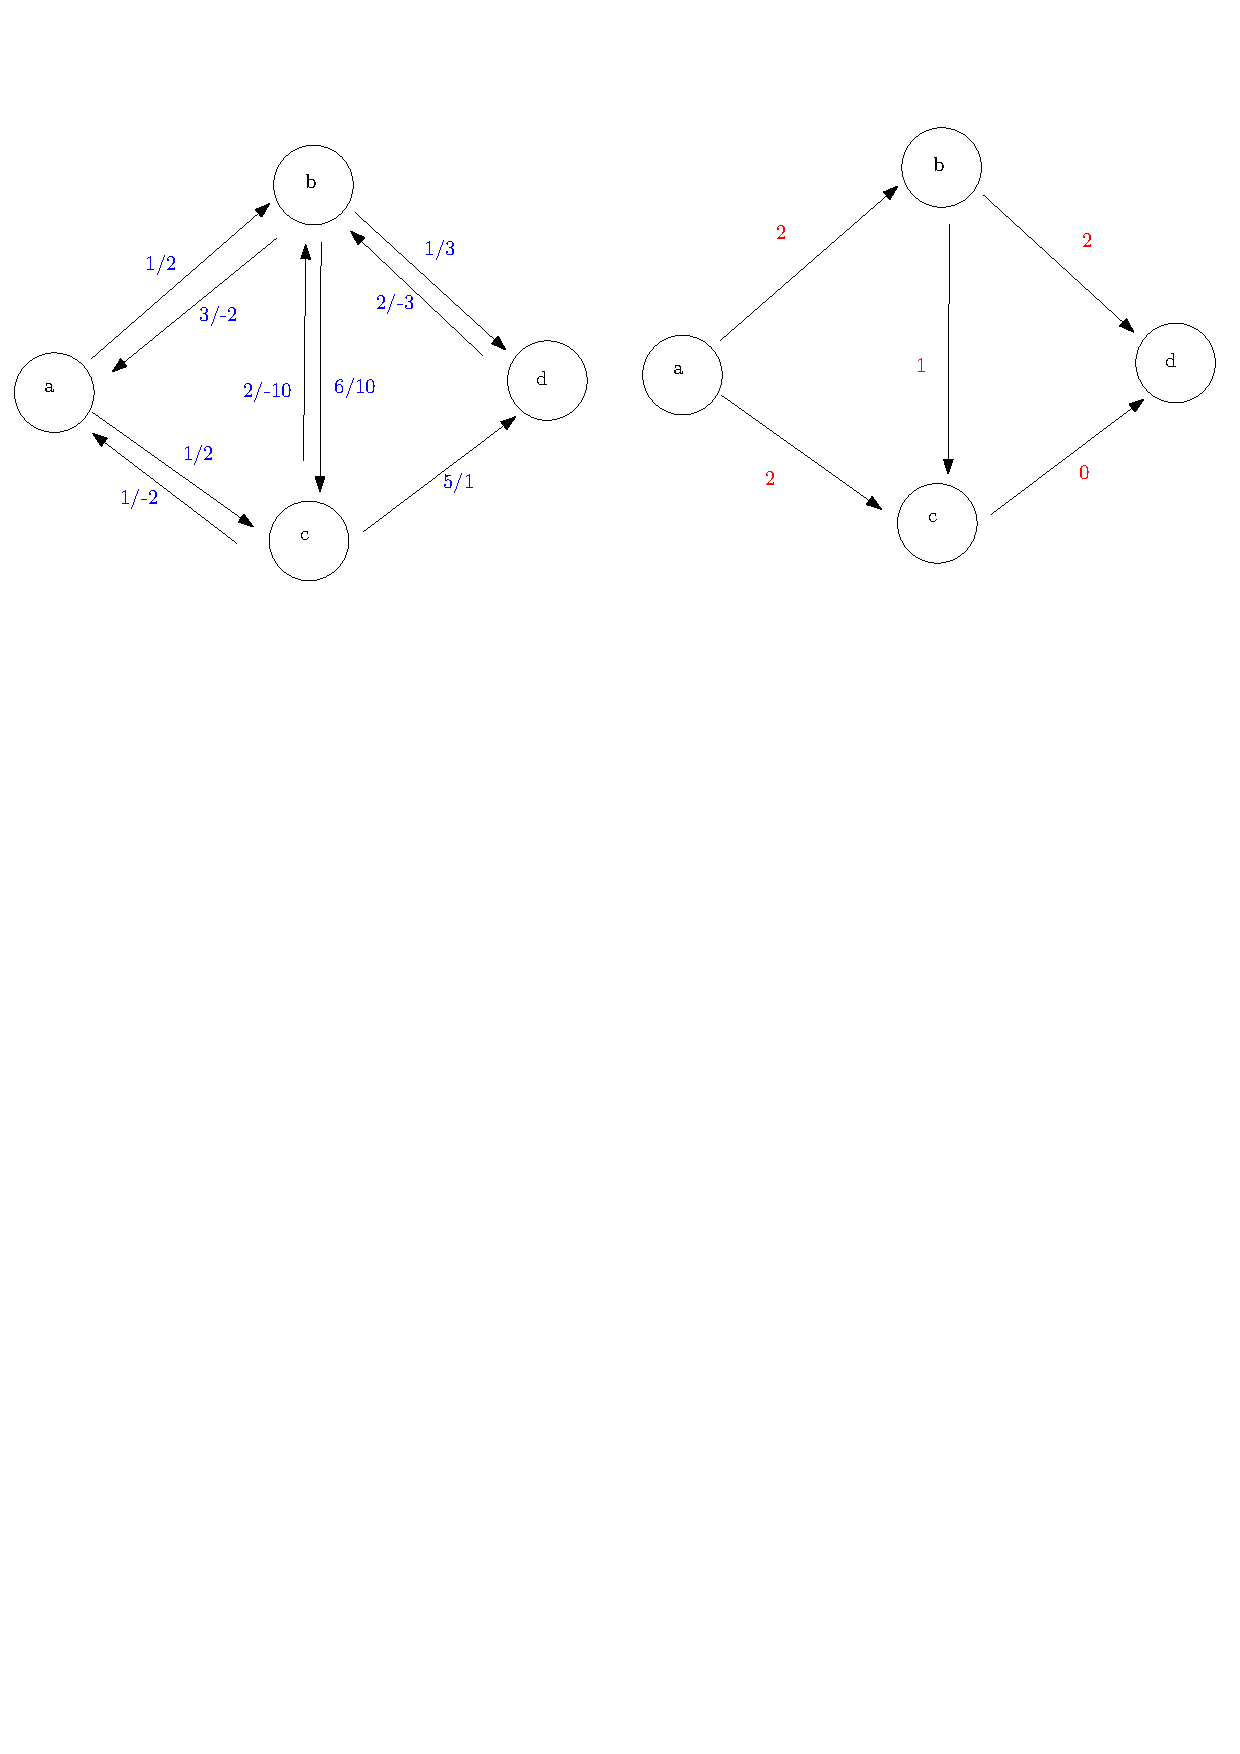
\includegraphics[width=\textwidth]{Figs/minCostFlow-Ex1-residual3}
\caption{Residual network for mcf instance and flow from Figure \ref{fig:minCostFlow-Ex1} (left). Resulting flow of cost 24 after sending one unit of flow along the negative cycle cbac (right).}\label{fig:minCostFlow-Ex1-residual}
\end{figure}

\begin{figure}
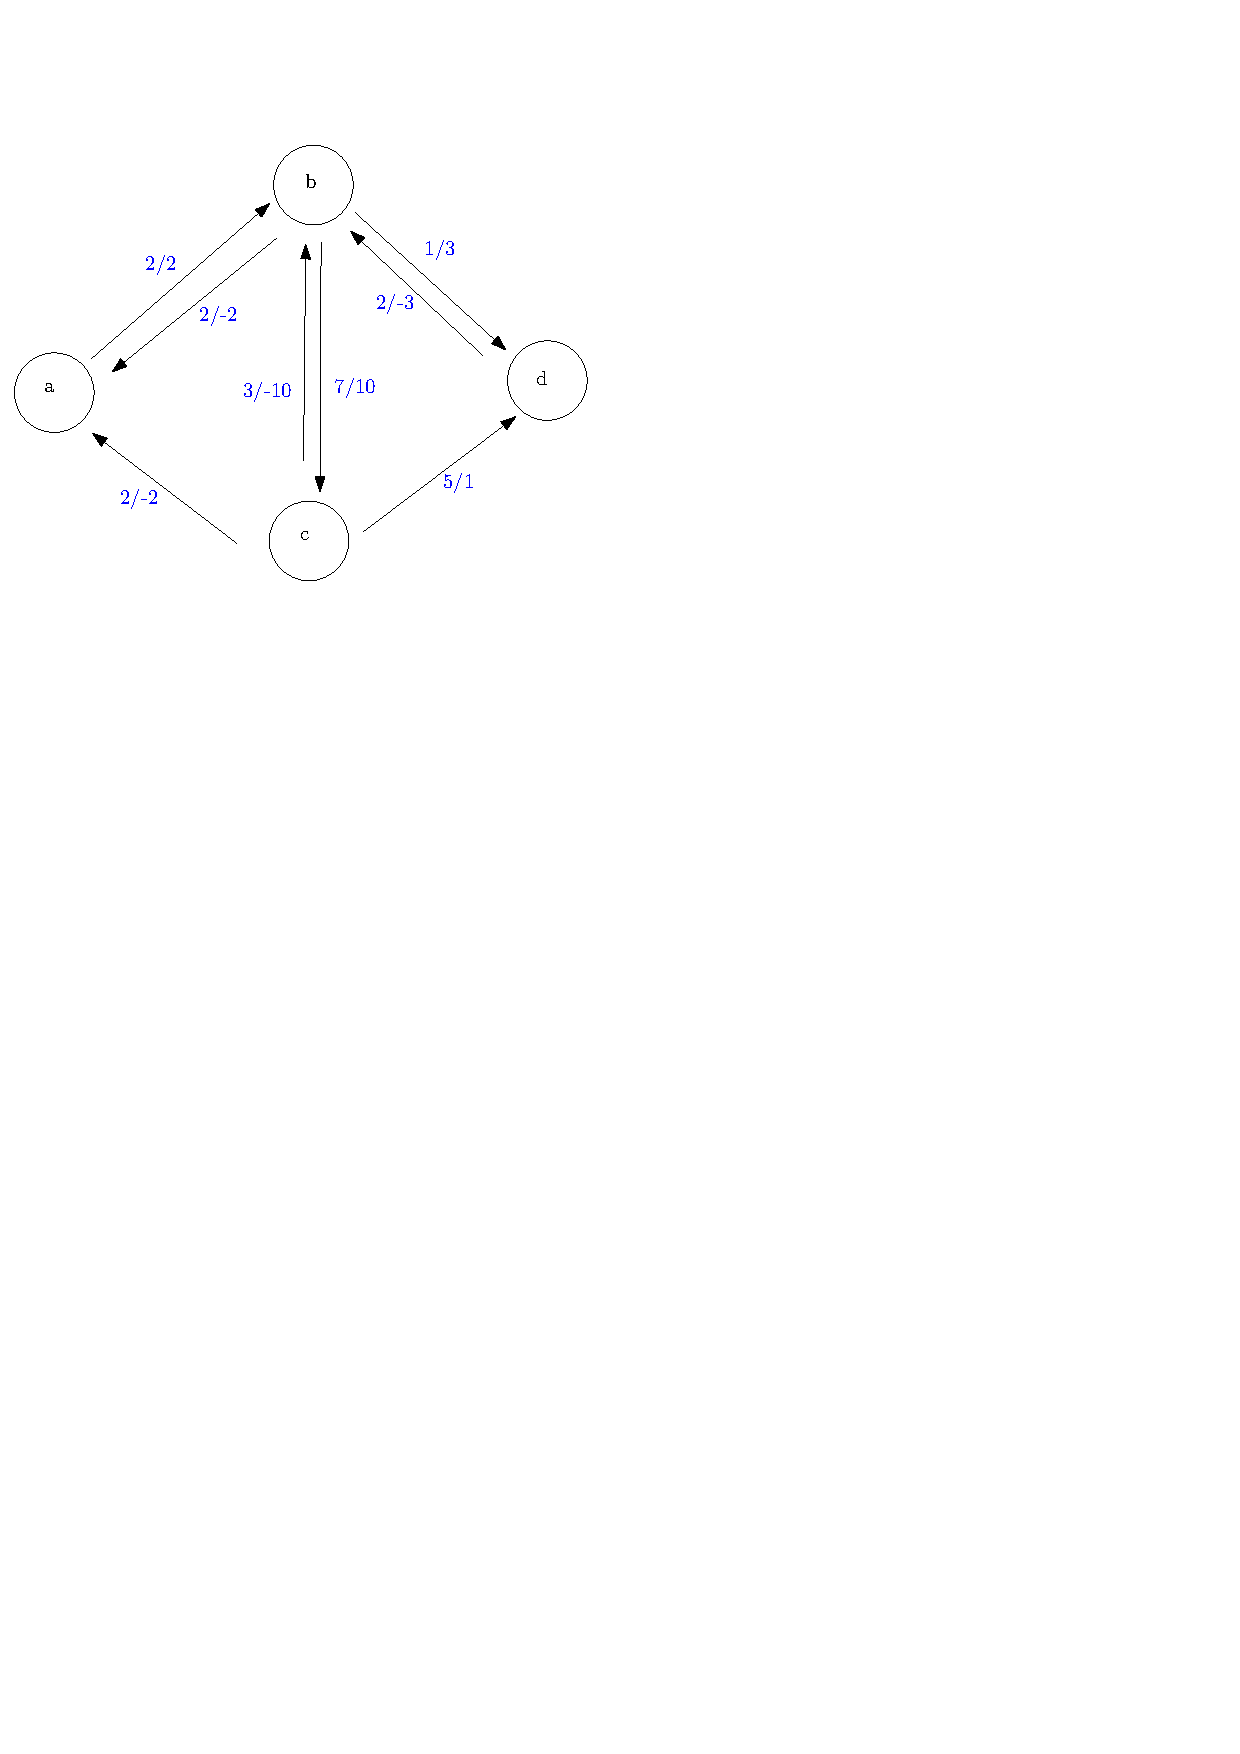
\includegraphics[width=0.5\textwidth]{Figs/minCostFlow-Ex1-residual2}
\caption{Final residual network without negative cycles.}\label{fig:minCostFlow-Ex1-residual2}
\end{figure}
While in our maxFlow algorithm we were looking for $s$-$t$-paths in this residual network, here we are looking for \emph{negative cycles}, that is a sequence of adjacent edges which ends up in the starting vertex and has negative cost in total. We send as much flow around this cycle as possible (as determined by the bottleneck edge capacity), hereby \emph{decreasing the total cost of the flow.}

In the residual network in Figure \ref{fig:minCostFlow-Ex1-residual}, left there exists a cycle $cbac$ of negativ cost; sending one unit of flow along this cycle (more is not possible due to the bottleneck edge $(a,c)$) decreases the total cost resulting in the flow in Figure \ref{fig:minCostFlow-Ex1-residual}, right.
As in Ford-Fulkerson we repeat this procedure until no negative cycles can be found in the residual network. As we will prove in the following, the resulting flow has to be optimal. \textcolor{blue}{\emph{(Algorithm aka. "`cycle canceling"')}}

\textcolor{blue}{\emph{This algorithm terminates as the initial cost is bounded by $`maxFLowValue' * |E| * 'maxCostOfAnEdge'$ and decreased by at least 1 in each round of cancelling negative cycles.}}

In Figure \ref{fig:minCostFlow-Ex1-residual2} we see the residual network for the updated flow. This network does not contain any negative cycle, so the flow is hopefully cost-optimal.

\begin{lemma}
Let $f$ be a feasible flow in $G$, $G_f$ the respective residual network. Then, $f$ is a minCost flow if and only if $G_f$ does not contain any negative cycle.
\end{lemma}
\begin{proof}
\textcolor{blue}{\emph{We need to prove '$\Rightarrow$' and '$\Leftarrow$'.}}

\textcolor{blue}{\emph{'$\Rightarrow$': Assume f is a minCost flow. To Show: there is no negative cycle in $G_f$. Assume otherwise, that is, $G_f$ has a negative cycle. Then send (at least 1 unit of) flow around that cycle, decreasing the total cost by at least 1. This is a contradiction to $f$ being a minCost flow.}}


The '$\Rightarrow$'-direction is trivial, so let us focus on the other direction and assume $G_f$ does not contain any negative cycle but $f$ is not a minCost flow. We will derive a contradiction hence proving the lemma.

'$\Leftarrow$': Let $f^*$ be a minCost flow and consider the flow difference $f'=f^*-f$  \textcolor{blue}{\emph{(for example of $f'$ see picture from 2013-11-05-1217)}}. We claim $f'$ has to contain a negative cycle  \textcolor{blue}{\emph{and this is also contained in $G_f$}}. Clearly we have $c(f')<0$ since $c(f^*)<c(f)$. Furthermore, note that for $f'$ flow conservation must hold, that is, at any $v\in V$ the inflow and the outflow of $f'$ balances out to $0$. \textcolor{blue}{\emph{It has to balance out, because a diffference flow cannot change the defficit or surplus of a node.}} Therefore, $f'$ must be decomposable into a set of one or more \emph{cycles}. Since the total cost of the cycles is negative, one of the cycles must have negative cost. Let that cycle be $C$; note that the flow described by $C$ can also be sent around in $G_f$, contradicting the fact that $G_f$ has no cycle of negative cost.
\end{proof}

So, as long as the current flow $f$ is not optimal, we will find a negative cycle in $G_f$, hence decreasing the cost of the flow by at least $1$ (for integral capacities and costs). Termination and correctness follow.

\subsubsection*{Detection of Negative Cycles}
How can we detect negative cycles in a graph $G(V,E,c)$? A naive way of doing so is to construct the following \emph{layered graph}:
we have $n$ layers where each layer contains the node set $v_1, \dots, v_n$. We have an edge between $v_i$ and $v_j$ in the next
layer if there is an edge $(v_i, v_j)\in E$ (of the same cost), see Figure \ref{fig:negCycle}. Now, we can compute shortest path distances for each $v_i$ in layer $1$ to the $v_i$ in the other layers in $O(mn)$ time each. If there is a negative cycle in $G$, it will be exhibited.
\begin{figure}
\begin{center}
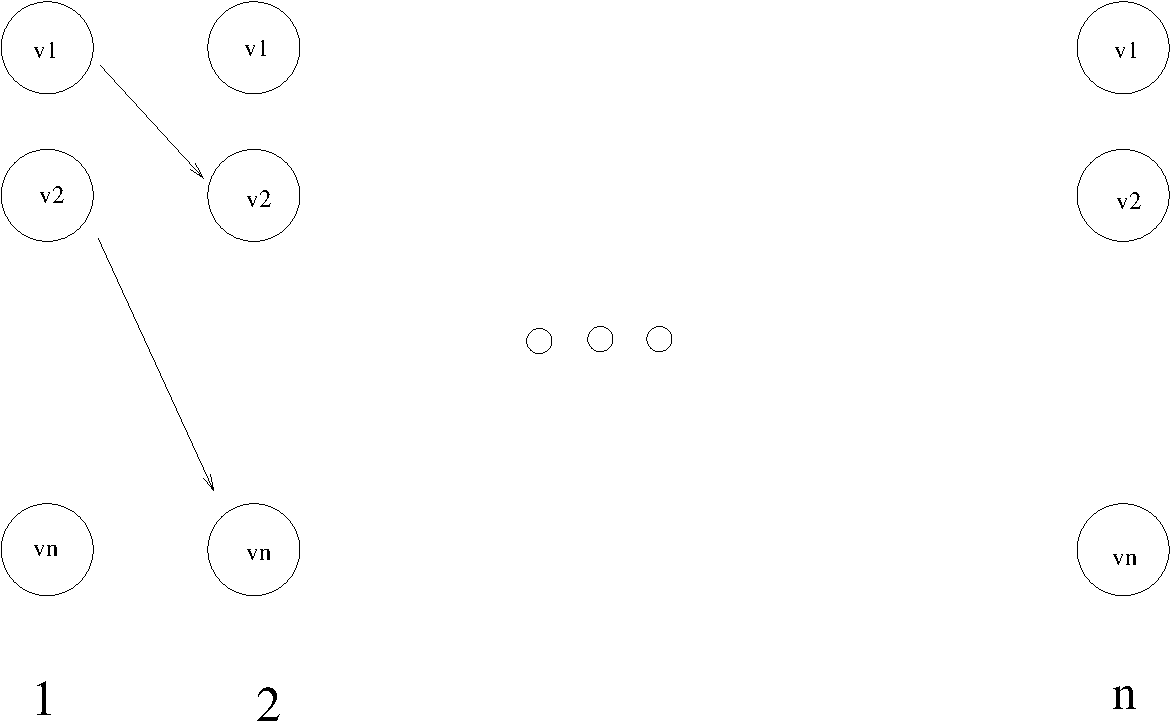
\includegraphics[width=0.5\textwidth]{Figs/negCycle.pdf}
\caption{Layered graph construction to detect negative cycles.}\label{fig:negCycle}
\end{center}
\end{figure}

While this naive approach requires $O(mn^2)$ steps it is also possible to employ Bellman-Ford and exhibit a negative cycle in time $O(mn)$ or conclude that no negative cycle exists.
In fact, when we always look for the negative cycle $C$ which minimizes $c(C)/|C|$, one can even prove that after polynomially many cycle detections the mincost flow has been found (similar to the maxFlow case where we used a specific rule to determine augmenting paths which guaranteed polynomial running time).

\subsubsection{MinCostFlow via Successive Shortest Paths (sketch)}
While the idea of cycle cancelling was to start with a \emph{feasible maxFlow} and decrease its cost by repeatedly identifying cycles of negative cost in the residual network, another strategy is to start with a zero flow and iteratively augment this flow while maintaining cost optimality. This is done by computing a  shortest augmenting path (\emph{wrt to the edge costs}) from some supply node to some demand node in the current residual network and sending as much flow as possible across that path. Then the supply and the demand of the respective nodes are reduced and the residual network is updated.
 Cost optimality (even for a non-maximal flow) is certified by absence of negative cycles in the residual network (we will argue that this is the case). Termination and construction of a feasible maxflow is guaranteed for the same reason as for the Ford-Fulkerson algorithm -- indeed, we can view this simply as a specific strategy for picking augmenting paths in the Ford-Fulkerson algorithm which happens to guarantee cost optimality.
 
How can we find the shortest path from some supply to some demand node? We construct a super source $s$ and connect this with outgoing edges of inifinite capacity and zero cost to all supply nodes, and a super sink $t$ which has incoming edges from all demand nodes (also with infinite capacity and zero cost). Then we compute a shortest path from $s$ to $t$ wrt to the edge costs e.g. using Bellman-Ford. 

\begin{figure}
\centering
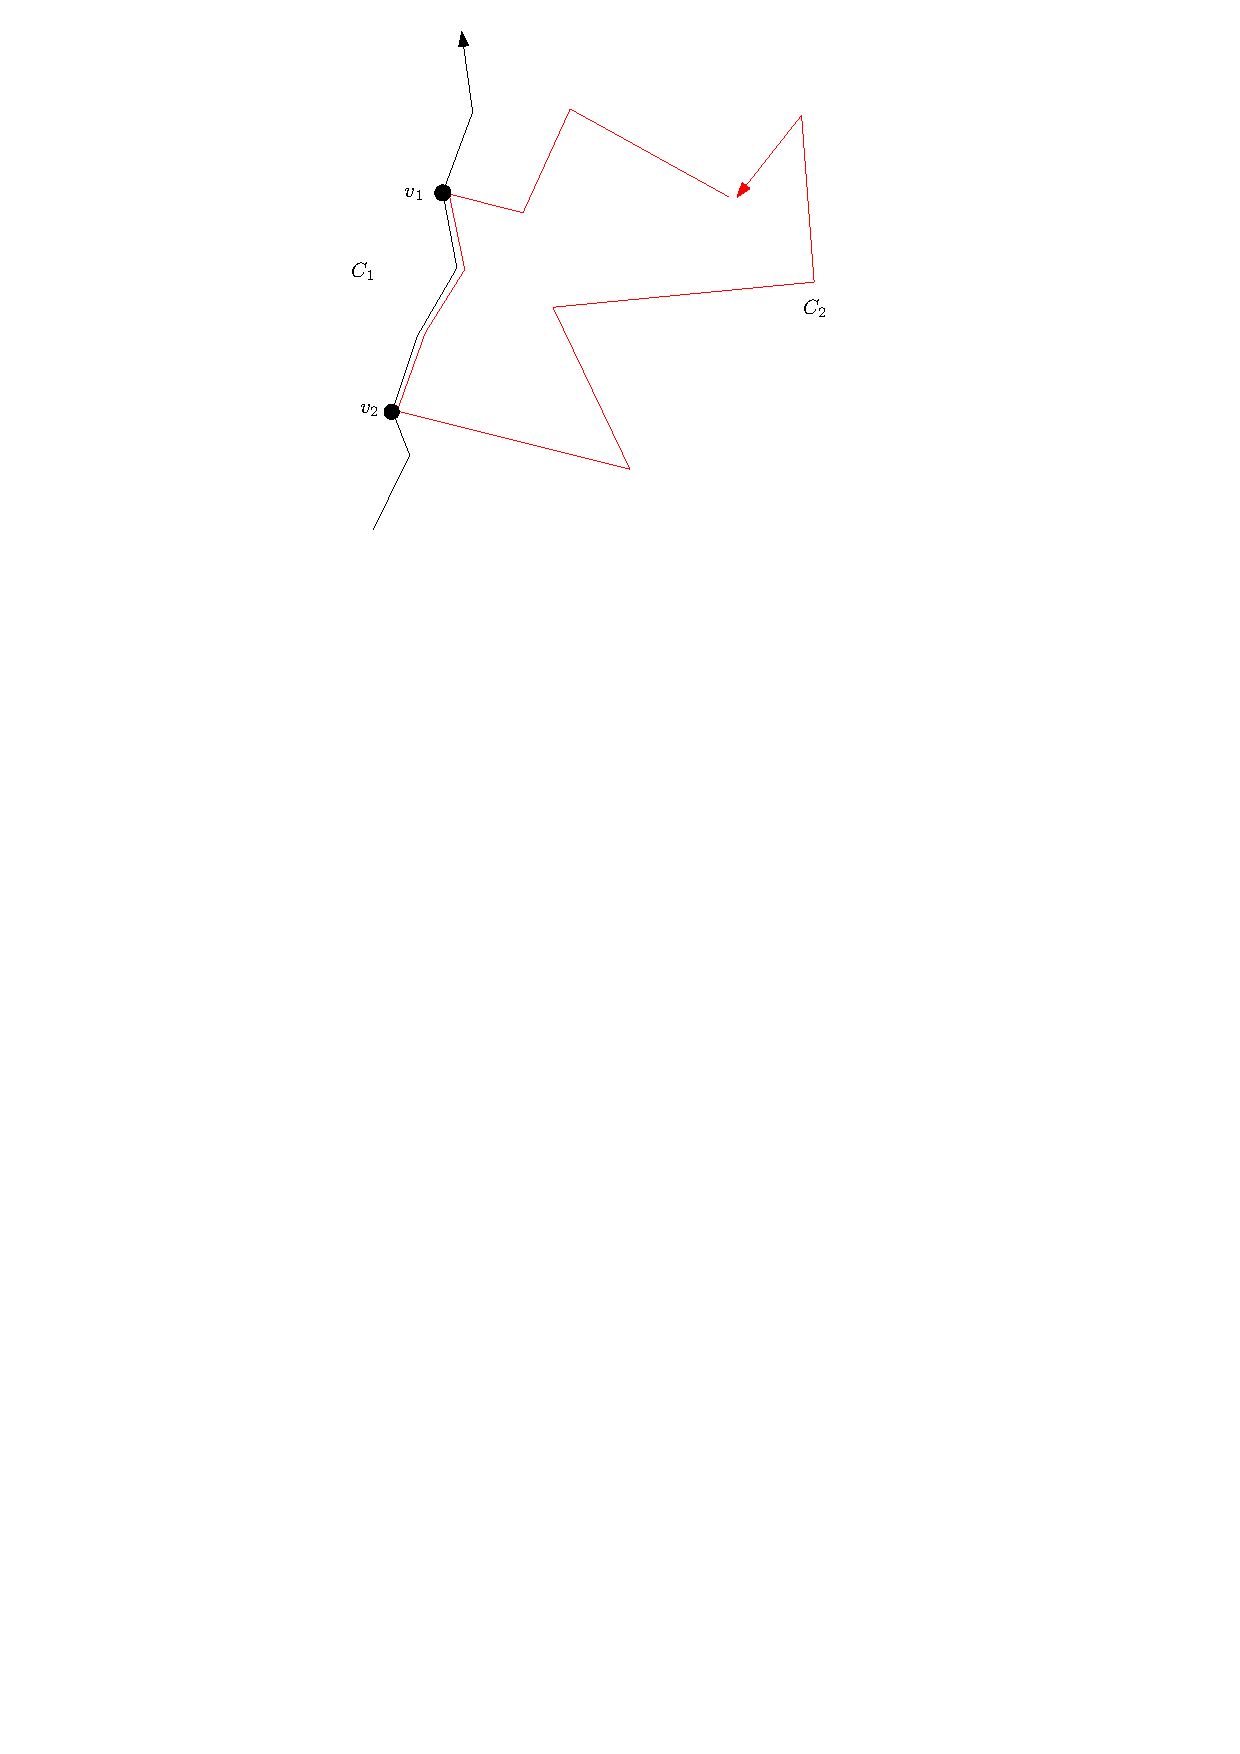
\includegraphics[width=0.4\textwidth]{Figs/SSP-noNegCyc.pdf}
\caption{Augmenting path in black, negative Cycle $C=C_1.C_2$. $C_1$ traverses the augmenting path between $v_2$ and $v_1$ in reverse direction (negative costs!).}\label{fig:SSPnoNegCyc}
\end{figure}
\textcolor{blue}{\emph{"`Claim: Residual networks occuring during execution of the algorithm never have a neagtive cycle."'}}
\textcolor{blue}{\emph{Consider first iteration, i.e. we have found shortest path (acc. to costs) in $G_f$ with $f=0$, i.e. in the original network.}}

How can we argue that after sending the maximum amount of flow across the identified augmenting path, the new residual network remains free of negative cycles? To that end, let us consider the first residual network (wrt to a zero flow) which has only positive edge costs. After augmentation, the only negative edge costs appear as reverse edges along the augmenting path. If after the augmentation a negative cycle $C$ exists, $C$ can be decomposed into paths $C_1$ and $C_2$ where $C_1$ starts and ends with negative cost edges and $C_2$ only contains positive cost edges. The cost of $C_1$ must be negative, the cost of $C_2$ positive and $|cost(C_1)|>|cost(C_2)|$. Assume $C_1$ starts in $v_1$ and ends in $v_2$.  W.l.o.g. $C_1$ only consists of a continuous reverse subpath from $v_1$ to $v_2$ of the augmenting path (needs some argument $\Rightarrow$ exercise), that is, its cost is the (negative) cost of a subpath from $v_2$ to $v_1$ in the augmenting path, see the illustration in Figure \ref{fig:SSPnoNegCyc} \textcolor{blue}{\emph{($cost(C_1) = - const(v_2 \rightarrow v_1$)}}. Observe that $C_2$ also yields a path from $v_2$ to $v_1$ with $|cost(C_2)|<|cost(C_1)| \textcolor{blue}{\emph{$= const(v_2 \rightarrow v_1)$}}$ which contradicts the fact that the reverse of $C_1$ was a shortest path in the first residual network. \textcolor{blue}{\emph{Hence $G_f$ cannot have a neagitve cycle. (only in the first augmentation)}} So we can be sure that after the first augmentation the respective residual network is free of negative cycles. 

\textcolor{blue}{\emph{This argument only holds for the first augmentation. Later there might be several negative-cost edges all over the $G_f$.}}How can we extend this observation to the following residual networks? Here, an old result by Johnson comes as a rescue:

\begin{theorem}[Johnson]
\textcolor{blue}{\emph{Idea: Transformation into a graph with only non-negative edges.}}Let $G(V,E,c)$ be a directed, weighted graph with possibly negative edge costs $c:E\rightarrow \mathbb{Z}$, but without negative cycles. \textcolor{blue}{\emph{(After first augmentation $G_f$ is of such structure.)}} Then there exists a potential function $\phi:V\rightarrow \mathbb{Z}$ such that the shifted edge costs $c'(v,w)=c(c,w)+\phi(v)-\phi(w)$ \textcolor{blue}{\emph{(oldCost + potentialOfV - potentialOfW)}} are always non-negative and shortest paths in $G(V,E,c)$ remain shortest paths in $G(V,E,c')$ and vice versa.
\end{theorem}

\begin{proof}
W.l.o.g. \textcolor{blue}{\emph{("`Without loss of generality"')}} assume that $\exists s\in V$ from which all other nodes in $G$ can be reached. If $G(V,E,c)$ does not contain negative cycles, shortest path distances from $s$ are well-defined and can be computed using e.g. Bellman-Ford in $O(mn)$ time. Let us then define $\phi(v):=d_s(v)$ for all $v\in V$, that is, simply the shortest path distance from $s$. First, observe that due to $d_s$ being shortest path distances, $\forall (v,w)\in E$ we have $d_s(w)\leq d_s(v)+c(v,w)$ \textcolor{blue}{\emph{"`the shortest path distance to $w$ is less or equal than the shortest distance to $v$ plus the const of $v$ to $w$"'}} (otherwise going from $s$ to $w$ via $v$ yields a path shorter than $d_s(w)$). This is equivalent to $d(v)-d(w)+c(v,w)\geq 0$ or in other words $\phi(v)-\phi(w)+c(v,w)=:c'(v,w)$, that is, the new edge cost function $c'$ is always non-negative. Second, consider some path $\pi=s \rightarrow v_0 \rightarrow v_1 \dots t$ in $G(V,E,c')$; the cost of the path is $\sum_{(v,w)\in \pi} c'(v,w)=\sum_{(v,w)\in \pi} \phi(v)-\phi(w)+c(v,w)=\phi(s)-\phi(t)+\sum_{(v,w)\in\pi}c(v,w)$, that is, its original cost plus the potential of the source minus the potential of the target. Since the latter two terms are invariant for different $s-t$-paths, shortest paths in $G(V,E,c)$ are shortest in $G(V,E,c')$ and vice versa.
\end{proof}


So we can turn the second residual network (after the first augmentation) again into a network which has only non-negative edge costs and repeat the argument. In fact, most descriptions of the successive shortest path approach for MinCostFlow immediately apply the respective potential changes in the algorithm -- they might obscure the basic idea of the algorithm, though. The transformation into a graph with non-negative edge costs also allows for the application of Dijkstra's algorithm for finding the shortest paths along which to augment the flow.


\subsection{Applications of Flow}
There are many other interesting real-world problems -- apart from direct flow problems -- that can be modeled as a flow optimization problem. In the following we give some examples. 

\subsubsection{s - t Shortest Path}
\textcolor{blue}{\emph{Problem: Given $G(V,E,c)$ and $s,t \in V$, find shortest (wrt. $c$) path from $s$ to $t$.}}

\textcolor{blue}{\emph{Solution: set $b(s)=1$, $b(t)=-1$, all capacities to 1, all edges costs remain $b(v)=0  \forall v\in V - \{s,t\}$}}

\textcolor{blue}{\emph{Similarily w can also solve ont-to-all (shortest paths from $s$ to all other nodes).}}

\subsubsection{transportation Problem}

\textcolor{blue}{\emph{$m$ facilities $f_1, f_2 \dots f_m$; each has $s_i$ units of some good. $n$ facilities $u_1, u_2 \dots f_n$; each of which has a demand.}}

\textcolor{blue}{\emph{...}}

\textcolor{blue}{\emph{see picture of 2013-11-07-1045}}

\textcolor{blue}{\emph{For $n=m$ and $s_i =1 \forall i$ and $d_j=1 \forall j$ this becomes the assignment problem. Wokrer $i$ can do job $j$ at cost $c_{i,j}$. How to assign jobs to workers (1:1) while minimizing the cost?}}

\subsubsection{Application of the assignment Problem}
\textcolor{blue}{\emph{Vodafone at any point in time knows the approx. location of ith cell phone users and at another point in time afurther approx. location. How to assign the locations in different time intervals to the same user and therefore trace the user or create a movement profile.}}

\textcolor{blue}{\emph{Solution to assignment problem yields correspondence of location over discrete time steps. iterate this and we get trajectories along which users ware moving.}}

\subsubsection{Airplane Mapping Problem}
\textcolor{blue}{\emph{Plane flying each day fixed route with $n$ hops: $v_1,v_2,v_3, \dots v_n$. Plane can carry $p$ passengers. Let $t_{ij}$ denote the number of passengers who want to travel from $v_i$ to $v_j$ and they are willing to pay some $f_{ij}$ for the journy ($i < j$). Goal is how to maximize the profit.}}

\textcolor{blue}{\emph{Picture from 2013-11-07-11:10}}

\textcolor{blue}{\emph{We introduce nodes $i,j$ reprecenting passengers who want to travel from $v_i$ to $v_j$. The supply $d(i_j):=t_{i,j}$. We add an edge of capacity $\infty$ and  cost from $f_{i,j}$ $i,j$ to $v_i$ and an edge of capacity $\infty$ and cost $0$ from $i,j$ to $v_j$. $v_i$ and $v_j$ are all connceted via edges of capa. $p$ and const $0$. the demant at a node $v_j$ is $\sum_i{t_{ij}}$. Computing the minCost-Flow yields the best (in terms of profit) choice for which passenger to take on board.}}

\textcolor{blue}{\emph{Pictures from 2013-11-14 in addition to ex 2.}}

\subsubsection{(MinCost) Bipartite Matching}
Consider a set of Jobs $J$ and a set of workers $W$ with $|J|=|W|=n$. Each worker $w\in W$, due to his qualification, is able to process a certain subset $J_w\subset J$ of tasks. Is it possible to find an assignment of jobs to workers such that every job is processed and no worker has to process more than one job?

This problem can be modelled as a maxFlow problem instance by creating a network with $V=W\cup J\cup\{s,t\}$ and edges $(w,j)$ of capacity $1$ between $w\in W$ and $j\in J$ if worker $w$ can process job $j$. Additionally we have capacity $1$ edges $(s,w)$ for all $w\in W$ and $(j,t)$ for all $j\in J$. A 1:1 assignment of jobs now exists iff the max flow from $s$ to $t$ is $n$.

A generalization of this problem where each job-worker pair has an associated processing time and the goal is to minimize the sum of processing times can be modelled as a minCostFlow problem.

\subsubsection{Edge Connectivity Edge-Disjoint Paths}
Given an undirected graph, its \emph{edge connectivity} $ec(G)$ is the minimal number of edges that need to be removed to make the graph disconnected. Clearly $ec(G)\leq \min deg(v)$, since removing all adjacent edges of a node makes $G$ disconnected. The edge connectivity of $G$ might be much smaller than the minimum degree of the nodes of $G$, though.

We can determine the edge connectivity by creating a network where each undirected edge is replaced by two directed edges of capacity $1$ (back and forth). We then compute the maxFlow from some fixed node $s$ to each $v\in V-\{s\}$. The minimum over all the flow values is the edge connectivity.

Similarly, for given $s$ and $t$ we might be interested in the number of \emph{edge disjoint} paths between $s$ and $t$. This number can be computed via a simple $s-t$ maxFlow computation when each edge has capacity $1$.

\subsubsection{01-matrices with given row and column sums}
Given two vectors $r\in \mathbb{N}^h$ and $c\in \mathbb{N}^w$, does their exist a matrix in $\{0,1\}^{h\times w}$ with the row sums given by $r$ and the column sums given by $w$?

Certainly, $\sum r_i=\sum c_j$ since the total number of $1$s in the matrix remains the same irrespectively of the way we count them. We construct a network consisting of $h+w+2$ nodes, named $s,x_1, \dots, x_h, y_1,\dots,y_w,t$. There is an edge $(s,x_i)$ of capacity $r_i$ for all $i=1,\dots,h$ and an edge $(y_j,t)$ of capacity $c_j$ for each $j=1,\dots, w$. Furthermore, we have $hw$ edges of capacity $1$ between any pair $(x_i, y_j)$ of nodes. If there is a flow of value $\sum r_i$ in this network, a $01$-matrix can be constructed by checking which edges $(x_i, y_j)$ actually bear a non-zero flow. On the other hand, if such a matrix exists, a suitable flow of value $\sum r_i$ can be generated.
\subsection{Exercises}
\Problem{1}
Use a flow formulation to determine the maximum number of \emph{node-disjoint} paths between two nodes $s$ and $t$ in an undirected network.

\Problem{2}
What is the intuitive meaning of the maxFlow/minCut theorem when applied to the maxFlow instance derived from the bipartite matching problem?

\Problem{3}
Describe maxFlow problem instance and a sequence of $\theta(C)$ augmentations, where $C$
is the maximum capacity of an edge in the network.

\Problem{4}
Describe a problem instance for the maxFlow problem \emph{with real capacities} and a sequence of augmentations which never lead to termination of the Ford-Fulkerson algorithm.

\newpage


\section{Linear Programming Basics}
\subsection{Real-World Motivation -- A Cheap but Healthy Diet}
One of the standard textbook examples for real-world applications of linear programming
is the following problem of determining a cheap but 'healthy' diet.

In our simplified model a human being lives a healthy life if he consumes  at least 11 units of carbohydrates, 7 units of proteins,
 and 5 units of fat each day (this might not be fully agreed upon by some nutritionists).
These ingredients can be acquired by eating \emph{meat} (one unit of which contains 1 unit of carbohydrates, 3 units of proteins and
5 units of fat), \emph{tofu} (2:2:0), \emph{bread} (4:1:0) or \emph{cheese} (1:4:2). These food items can be bought in the local
supermarket for 7 EUR per unit of meat, 3 EUR/Tofu, 2 EUR/Bread, 4 EUR/Cheese. The goal is to minimize the daily cost of
a healthy nutrition. 

We can formalize this goal mathematically by introducing variables $x_m, x_t, x_b, x_c$ representing the
units of meat, tofu, bread and cheese that we are to buy in the supermarket and defining the following
\emph{objective function} 
\[
	7 x_m +3 x_t + 2 x_b +4 x_c
\]
which reflects the cost of our shopping spree and which is to be \emph{minimized} under
the following constraints:
\begin{itemize}
\item $1 x_m + 2 x_t + 4 x_b +1 x_c \geq 11$ which expresses the need for at least 11 units of carbohydrates per day \textcolor{blue}{\emph{(carb. constraint)}}
\item $3 x_m + 2 x_t + 1 x_b + 4 x_c \geq 7$ (at least 7 units of proteins per day)\textcolor{blue}{\emph{(protein constraint)}}
\item $5 x_m + 0 x_t + 0 x_b + 2 x_c \geq 5$ (at least 5 units of fat per day)\textcolor{blue}{\emph{(fat constraint)}}
\end{itemize}
Furthermore we can only purchase non-negative amounts of food, so in summary we can 
specify our optimization problem as the following \emph{linear program}:

\[
\begin{matrix}
	\min	& 7 x_m	&+& 3 x_t&+& 2 x_b&+&4 x_c&&\\  
	\mbox{s.t. \textcolor{blue}{\emph{(subject to)}}}	& 1 x_m &+& 2 x_t&+& 4 x_b&+&1 x_c&\geq&11\\
			& 3 x_m &+& 2 x_t&+& 1 x_b&+&4 x_c&\geq& 7\\
	           	& 5 x_m &+& 0 x_t&+& 0 x_b&+&2 x_c&\geq& 5\\
			& x_i\geq 0\\
\end{matrix}
\]

The objective function as well as the constraints are \emph{linear} in the variables,
hence the name linear program.

In the remainder of this section we will have a closer look at such linear programs
and devise algorithms for finding optimal solutions to them if they exist.

\textcolor{blue}{\emph{``If the solution is restriced to integral, then it cannot be solved in polynomial time. For now we stick to the fact, that the solution can also be non-integral."}}


\subsection{Linear Programs -- Standard Form}
\label{sec:standard form}
Depending on the concrete application context, one can imagine that sometimes the linear
objective function is to be \emph{maximized} instead of minimized, or some of the 
linear constraints are not of a $\geq$-type, but of a $\leq$-type or even equalities.
It is convenient for the following exposition to assume that our linear program has the
following form:

\[
\begin{matrix}
	\max	& c_1 x_1 &+& c_2 x_2 &+& \dots &+& c_n x_n&&\\  
	\mbox{s.t.}	& a_{11} x_1 &+& a_{12} x_2&+& \dots &+&a_{1n} x_n&\leq&b_1\\
			& a_{21} x_1 &+& a_{22} x_2&+& \dots &+&a_{2n} x_n&\leq&b_2\\
			& ..	&&&&&&&&\\
			& a_{m1} x_1 &+& a_{m2} x_2&+& \dots &+&a_{mn} x_n&\leq&b_m\\
\end{matrix}
\]

Here we have a \emph{maximization} problem in $n$ variables $x_1, \dots x_n$, 
$n$ coefficients $c$ for these variables in the objective function, and $m$ constraints 
given as a matrix $A\in\mathbb{R}^{m \times n}$ and a vector $b\in\mathbb{R}^m$.
The $j$-th constraint is then 
\[
	\sum_{i=1}^n a_{ji}\leq b_j
\]

It is not hard to see that one can transform any linear program into this standard form
(see exercises).

\subsubsection{Geometric Interpretation}
The above standard form can be easily interpreted geometrically.
Figure \ref{fig:GeomIntuition} shows a simple linear program with two variables
and its visualization in the Euclidean plane. 

Here we have two  variables $x$ and $y$ which are to obey a set of $4$ constraints. 
Each constraint defines a \emph{halfplane} \textcolor{blue}{\emph{(indicated by /////// )}}in which all \emph{feasible solutions}
(all allowed assignments of values to $x$ and $y$) lie. The intersection of the
$4$ halfplanes defines a polyhedron (an intersection of halfplanes/spaces),
the so-called \emph{feasible region} of the LP (hatched area in the figure). 
Being the intersection of several
\emph{convex sets}, the feasible region itself is also convex. Each \emph{corner} or \emph{vertex} of the feasible region is defined by the intersection of (at least) two lines bounding the halfplanes of respective constraints.

What we are interested in is a point of the feasible region which maximizes the given objective
function. If the objective function is \emph{linear} this corresponds to finding an \emph{extreme
point} of the feasible region in a certain direction which is specified by the coefficients
of the objective function. In this concrete example, the objective function is $\max x+y$, that
is, we are looking for a feasible point that is furthest in direction 
$\left( \begin{array}{c} 
1\\ 
1\\ 
\end{array}
\right)$ (the blue arrow in the figure). 

In figure \ref{fig:GeomIntuition} we have depicted in red the isolines of the objective function, that is, the
set of all points which have the same objective function value. The set of all points with objective function $0$ is
a line with slope $-1$ passing through the origin. The set of all points with objective function $5$ is a 
line passing through points $(0,5)$ and $(5,0)$ and so on. The point of the feasible region
with maximum objective function value is the corner $(7, 3.5)$.

In dimensions higher than $2$, the halfplanes become \emph{halfspaces}, the feasible region is a polyhedron defined as the intersection of a set of halfspaces. Each corner of the feasible region of a linear program with $d$ variables (that is, in $d$ dimensions) is defined by the intersection of $d$ hyperplanes bounding $d$ halfspaces of respective constraints.

\begin{figure}[t]
\begin{minipage}{4cm}
\[
\begin{matrix}
	\max		& x	&+	y	&&\\ 
	\mbox{s.t.}	&-x	&	-y	&\leq&-3\\ 
			&0.5x	&	+y	&\leq&7\\ 
			&0.5x	&	-y	& \leq&0\\
			&-0.5x	&	+y	& \leq&3\\
\end{matrix}
\]
\end{minipage}
\hspace{1cm}
\begin{minipage}{10cm}
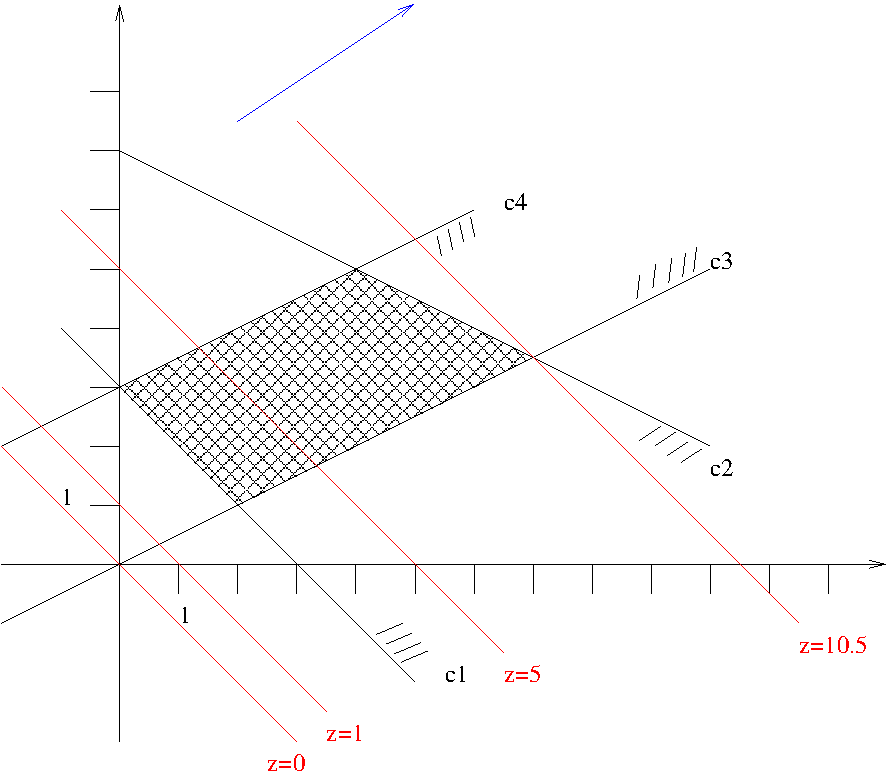
\includegraphics[width=9cm]{Figs/GeomIntuition.pdf}
\end{minipage}
\caption{A simple linear program in two dimensions and its visualization in the
	Euclidean plane.\label{fig:GeomIntuition}}
\end{figure}

Note that it is well possible that the feasible region -- the intersection
of the halfspaces given by the constraints -- is empty or unbound. In that case, no solution
exists which satisfies all the constraints, we call the linear program \emph{infeasible}.

\begin{lemma}
If the feasible region is a bounded, non-empty polyhedron, 
the maximum objective function value is 	attained at a corner (also called \emph{vertex})
 of the polyhedron.
\end{lemma}
{\bf Proof:} Follows from the convexity of the polyhedron and the 
linearity of the objective function.

There might be more than one feasible point with maximal objective function value. Think
of respective examples in $2$ and $3$ dimensions.

\subsubsection{Solve Max-Flow with Linear Programming}

\textcolor{blue}{\emph{1. Give each edge a variable $x_1, x_2, x_3, \dots\, x_m$ 2. objective function: max edges leaving $s$ 3. As constraints let edges be less or equal capacities of edges and formaulate conservation constraint as a equation.}}


\subsection{The (Primal) Simplex Algorithm}
Let us now turn to the problem of actually \emph{finding} an optimal vertex of the polyhedron for a given objective function. We will first explain the algorithm in $2$ dimensions and then extend it to higher dimensions.

Without loss of generality let us assume that the objective is to find the \emph{lowest corner} of the feasible region (otherwise rotate the whole problem instance). The high-level strategy of the Simplex algorithm is quite simple:
starting with some corner of the feasible region, jump to a neighboring \emph{lower} corner of the feasible region until all neighboring corners are not below the current corner, see Figure \ref{fig:simplexPrimal}. In two dimensions, there is only one vertex (the highest one) where there is an actual choice which corner to visit next. The other corners -- except the ones with minimum $y$-coordinate -- have exactly one neighboring corner which is lower. \textcolor{blue}{\emph{Picture form 2013-11-19-12:17}}

In Figure \ref{fig:simplexPrimal} we also see an example where more than two bounding lines intersect in a vertex (leftmost corner of the feasible region). This is called a \emph{primal degeneracy} and will lead to some complications later on for the Simplex algorithm.


\begin{figure}
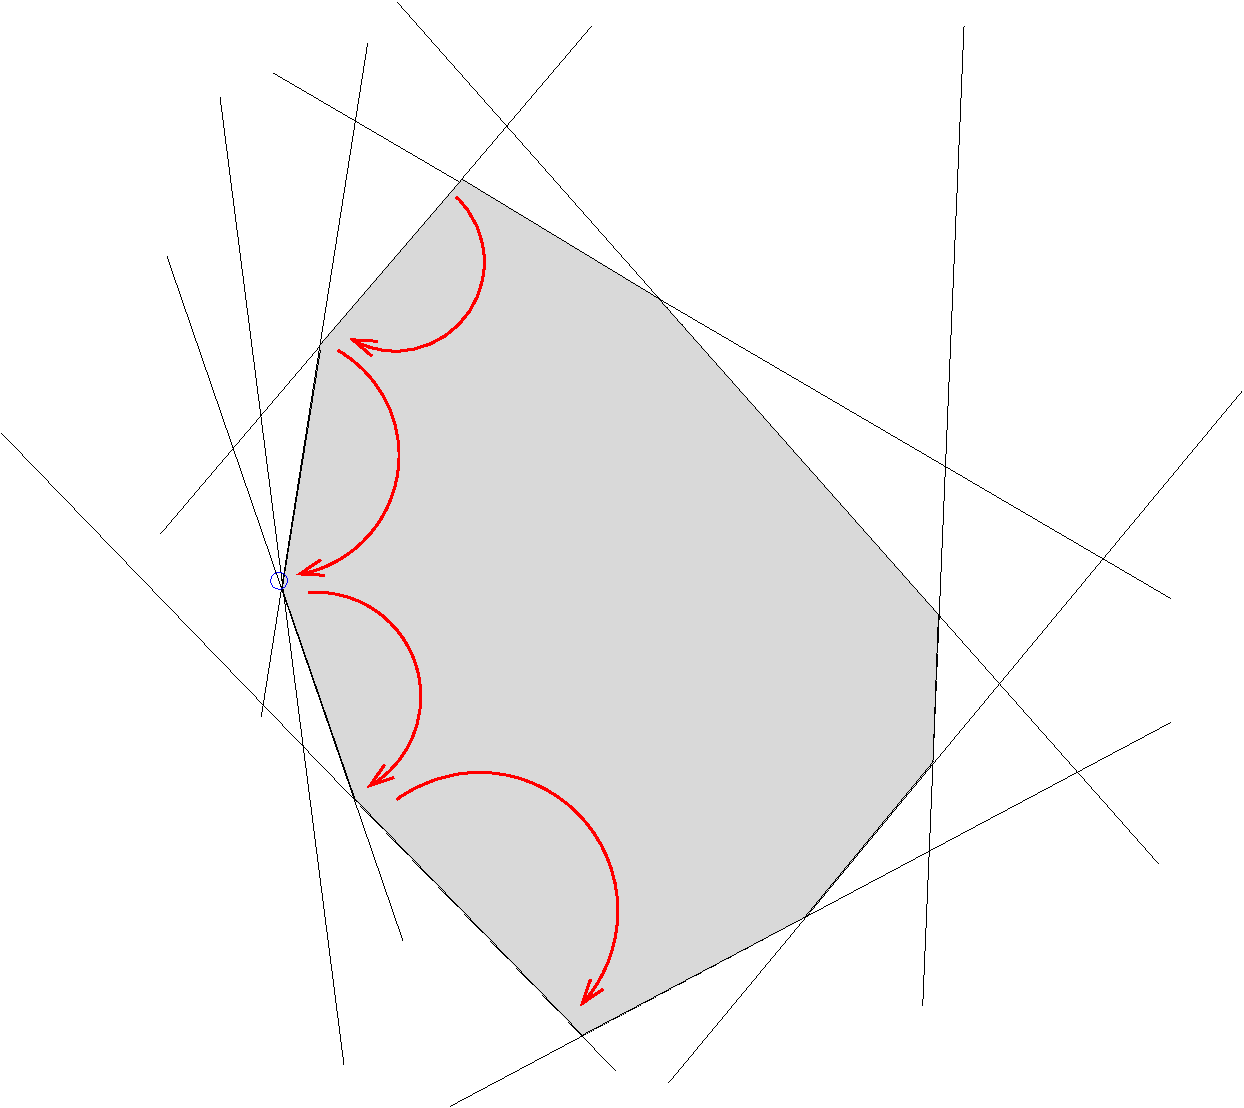
\includegraphics[width=10cm]{Figs/simplexPrimal.pdf}
\caption{Primal Simplex algorithm: jumping from corner to lower corner.}\label{fig:simplexPrimal}
\end{figure}




\subsubsection{Simplex Algorithm in Higher Dimensions}
Translating the basic idea of the Simplex algorithm to higher dimensions is quite straightforward. In $d$ dimensions, a corner of the feasible region is defined by the intersection of $d$ hyperplanes bounding the respective halfspaces corresponding to the constraints (in $\mathbb{R}^3$, three planes in general position intersect in a point). The $d$ hyperplanes defining a vertex/corner are also called a \emph{basis}. The basic strategy remains the same, starting at a corner of the feasible region (defined by $d$ constraints) we keep jumping to adjacent lower corners until there is no neighboring corner below the current curner.

From the description it should be clear that the Simplex algorithm always terminates since for a linear program with $d$ variables and $n$ constraints there can be at most $n\choose d$ corners of the feasible region. As we never visit a corner twice the Simplex algorithm has to terminate after at most $n \choose d$ 'jumps'. Due to convexity of the feasible region, this strategy always leads to the optimal/lowest vertex.

\subsubsection{Making things more concrete}
While the high-level description of the Simplex algorithm seems quite straightforward, there are a few issues which have not been discussed so far:
\begin{itemize}
\item how to compute the corner defined by a basis of $d$ (linearly independent) constraints?
\item how to find an initial \emph{feasible} corner to start the Simplex algorithm from?
\item given a corner, how to find a neighboring \emph{lower} feasible corner if such exists (pivot step)?
\end{itemize}

Consider $d$ constraints $a_i^T x \leq b_i$, $i=1,\dots, d$; the vertex defined by these constraints is the point which satisfies all the constraints with equality, its coordinates can be computed by simply solving the following system of linear equations:
\[
	\mat{a_{11} & \dots & a_{1d} \\ \dots & \dots & \dots \\ a_{d1} & \dots & a_{dd}} x 
		 = \mat{b_1\\ \vdots \\ b_d}
\]

Postponing the problem of finding an initial feasible corner to the exercises, let us now see how we can actually jump from one feasible corner to another, lower feasible corner. This operation is called the \emph{pivot step} and its choice is of great importance for the performance of the Simplex algorithm.

\paragraph*{Pivoting}
Consider a feasible vertex $v'$ defined by $d$ constraints. There are $d$ halflines/rays (each defined by the intersection of $d-1$ constraints) emanating from $v$ on the boundary of the feasible region. We will try to follow one of those rays to get to a lower feasible vertex (which shares $d-1$ constraints with vertex $v$).

Let us first try to figure out which of the $d-1$ halflines to follow to improve our objective function value.
Our current solution is given by $d$ constraints $a_1^Tx\leq b_1 \dots a_d^Tx \leq b_d$. We can write
this system of inequalities as equalities by introducing slack variables $s=(s_1,\dots s_d)\in \setR^d_{\geq0}$:
\[
	\mat{a_{11} & \dots & a_{1d} \\ \dots & \dots & \dots \\ a_{d1} & \dots & a_{dd}} x 
		+ \mat{s_1\\ \vdots \\ s_d} = \mat{b_1\\ \vdots \\ b_d}
\]
We will write this as $A_B x + s = b_B$ in short. The coordinates of the current vertex are determined as 
\[
	x=A_B^{-1}b_B - A_B^{-1}s	
\]
with $s=(0,\dots,0)$, i.e. all $d$ constraints are tight. Moving away from one constraint corresponds to 
increasing its slack variable from zero to some positive value. We want to figure out which slack variable
we can increase to get a higher objective function value. For the objective function we have:
\[
	c^Tx= c^T(A_B^{-1}b_B - A_B^{-1}s)= c^T x' - \alpha_1 s_1 - \dots - \alpha_d s_d
\]
that means expressed in dependence on $s$, the objective function value is a constant (the value at our current
vertex position) and a sum of $s_i$ variables with respective coefficients. If we have for one $i$ 
$\alpha_i<0$, then increasing this slack variable -- i.e. moving away from the corresponding constraint and
sliding along the half-line determined by the remaining constraints -- improves the objective function.
If no such $i$ exists, all neighboring vertices are not below the current vertex.

Now assume we have found a constraint $a_i^T x \leq b_i$
which is going to leave the basis (as we can increase the objective function value thereby). 
It remains to find the constraint which
blocks this movement (if no such constraint exists, the problem is clearly unbounded).

$x'=A_B^{-1}b_B$ is the current vertex, choosing $x''=A_B^{-1}b_B - (A_B^{-1})_{\cdot i}$ (this is a point moved
one unit in the direction we have just determined), we can move 
on the improving ray  ($\lambda\geq 0$)
\[
	\overrightarrow{r}=x' + \lambda \cdot {(x''-x')}
			= x' - \lambda (A_B^{-1})_{\cdot i}
\]
and ask by which other constraint $j$ this movement is blocked first.
We can plug in a point $r(\lambda)$ on the ray in every constraint $l$:
\[
	a_l^{T}(x'-\lambda (A_B^{-1})_{\cdot i})\leq b_l
\]
\[
\Leftrightarrow	a_l^{T}x'-\lambda a_l^{T}(A_B^{-1})_{\cdot i})\leq b_l
\]
If $a_l^{T}(A_B^{-1})_{\cdot i})\geq0$ this constraint will never block our movement, otherwise
we obtain the following bound on $\lambda$:
\[
	\lambda \leq \frac{b_l - a_l^{T}x'}{-a_l^{T}(A_B^{-1})_{\cdot i})}
\]
If no constraint gives a bound on our movement, the problem is unconstrained, otherwise the constraint $j$
which determines the smallest upper bound on $\lambda$ is the first constraint hit when moving along
$\overrightarrow{r}$. This constraint enters the basis in exchange for constraint $i$.

\subparagraph*{Pivoting Strategies}
In particular for higher dimensional problems, there are typically \emph{several} constraints for whom moving away from increases the objective function value. There are many strategies to decide which constraint should leave the basis \textcolor{blue}{\emph{(``which ray to follow'')}}: \emph{the rule of steepest ascent} for example chooses to follow the ray which improves the objective function value at the highest rate; \textcolor{blue}{\emph{pick the ray where we can go down furthest;}} \emph{randomly choosing an improving ray} is another strategy (not as bad as it sounds).

Unfortunately, no strategy is known which guarantees a polynomial number of steps to reach the optimum/lowest vertex. Even worse, for many deterministic pivot rules, there are examples where an exponential number of steps are necessary to reach the optimum (the Klee-Minty cube is a well-known example -- google it!). \textcolor{blue}{\emph{In practive they perform very well though.}}


\subparagraph*{Basis Cycling and Bland's Rule}

To make things even worse, for many deterministic pivoting strategies there are examples where the Simplex algorithm does \emph{not} terminate at all! This can happen when $d'>d$ constraints intersect in a corner. Here, a naive pivoting strategy might lead to a cycling of the bases never leaving that corner. Bland's rule (google that!) guarantees that after a finite number of steps, the corner is left for a better corner. As applying Bland's rule all the time in practice often leads to worse running times of the Simplex algorithm (more steps), in real-world applicaitons people use rules like the one of steepest ascent and only if cycling is suspected (when the Simplex algorithm stays at the same corner for several steps), Bland's rule is employed until the vertex has been left.

Alternatively, one might remove degeneracies by slightly perturbing constraints such that no $d+1$ constraints intersect in a single point.
\textcolor{blue}{\emph{In higher dimension it can happen, that by always exchanging the constraints the algorithm stays at that one corner and dous not make any progress. (only with $d'>d$ constraints)}}

\subsection{Duality}
One very powerful concept in the context of linear programming is \emph{duality}. Let us first look at it in an abstract way and later try to provide some intuition.

Consider a linear program in standard form:

\[
\begin{matrix}
	\max	& c_1 x_1 &+& c_2 x_2 &+& \dots &+& c_n x_n&&\\  
	\mbox{s.t.}	& a_{11} x_1 &+& a_{12} x_2&+& \dots &+&a_{1n} x_n&\leq&b_1\\
			& a_{21} x_1 &+& a_{22} x_2&+& \dots &+&a_{2n} x_n&\leq&b_2\\
			& ..	&&&&&&&&\\
			& a_{m1} x_1 &+& a_{m2} x_2&+& \dots &+&a_{mn} x_n&\leq&b_m\\
\end{matrix}
\]

or more concretely the following linear program (a slight modification of the LP from Figure \ref{fig:GeomIntuition}):
\[
\begin{matrix}
	\max		& x	&+	y	&&\\ 
	\mbox{s.t.}	&-x	&	-y	&\leq&-3\\ 
			&0.5x	&	+y	&\leq&7\\ 
			&0.5x	&	-y	& \leq&0\\
			&-0.5x	&	+y	& \leq&3\\
			&	x	&		& \leq&6\\
\end{matrix}
\]

We could use the Simplex algorithm to solve this LP, but is it possible to give any upper bounds on the objective function value of the optimum solution beforehand?
Consider the two constraints $0.5x+y\leq 7$ and $0.5x-y\leq 0$. We could multiply the first constraint
by $1.5$ and the second constraint by $0.5$ without invalidating them and obtain $0.75x+1.5y\leq 10.5$ and $0.25x-0.5y\leq 0$. Adding these two constraints we get $x+y\leq 10.5$, that is, an upper bound of $10.5$ for the objective function \textcolor{blue}{\emph{(``which is better than 11 '')}}. In this case, this is not the best bound possible, though, since combining
the constraint $0.5x+y\leq 7$ with a multiplier of $1.0$ and the constraint $x\leq 6$ with a multiplier of $0.5$ yields an upper bound \textcolor{blue}{\emph{(by adding them up)}} of $10$ which happens to be the objective function value of the optimum solution.

A natural strategy to obtain upper bounds on the objective function value is to combine constraints by weighting and adding such that in the sum the coefficients of the variables match the coefficents of the objective function. Note that one better only uses \emph{positive} factors for weighting since multiplication with a negative number turns the $\leq$ into a $\geq$ in the inequality, which renders the obtained 'upper bounds' invalid. More formally we can define the following \emph{dual problem} which formalizes this search for the best upper bound:

\[
\begin{matrix}
	\min& b_1 y_1 &+& b_2 y_2 &+& \dots &+& b_m y_m&&\\  
	\mbox{s.t.}	& a_{11} y_1 &+& a_{21} y_2&+& \dots &+&a_{m1} y_m&=&c_1\\
			& a_{12} y_1 &+& a_{22} y_2&+& \dots &+&a_{m2} y_m&=&c_2\\
			& ..	&&&&&&&&\\
			& a_{1n} y_1 &+& a_{2n} y_2&+& \dots &+&a_{mn} y_m&=&c_n\\
			& y_i\geq 0\\
\end{matrix}
\]
Essentially we have a (positive!) multiplier $y_i$ for each (primal) constraint, $i=1,\dots m$. The multipliers should always be chosen such that the summed coefficients match the coefficients of the objective function; amongst all such multipliers we are looking for the combination which yields the best, that is, the \emph{lowest} upper bound. The discussion so far should has made clear that any feasible solution to this \emph{dual linear program} indeed is an upper bound for the primal linear program. This is also called \emph{weak duality}.

\textcolor{blue}{\emph{We try to find non-negative multipliers for the constraints such that adding the multiplied constraints yield the same coefficiant on the left hand side as the objective function and the right hand side is as small as possible.}}

In fact, it turns out that the best upper bound that can be achieved using the dual LP always matches \emph{exactly} the objective function value of the optimum solution in the primal LP. This is called \emph{strong duality}.

\textcolor{blue}{\emph{The primal LP problem is a maximization problem and the dual LP problem is a minimization problem. The optimal objective function value of the duality problem is at least as large as the optimal objective function value of the primal function.}}

\textcolor{blue}{\emph{\textbf{In Short:} Primal: $\max c^Tx$ with $Ax \leq b"$; Dual: $\min b^Ty$ with $A^Ty = c, y \geq 0$}}

\paragraph*{Economic Interpretation of the dual}
Recall our diet-LP from the introduction

\[
\begin{matrix}
	\min	& 7 x_m	&+& 3 x_t&+& 2 x_b&+&4 x_c&&\\  
	\mbox{s.t.}	& 1 x_m &+& 2 x_t&+& 4 x_b&+&1 x_c&\geq&11\\
			& 3 x_m &+& 2 x_t&+& 1 x_b&+&4 x_c&\geq& 7\\
	           	& 5 x_m &+& 0 x_t&+& 0 x_b&+&2 x_c&\geq& 5\\
			& x_i\geq 0\\
\end{matrix}
\]

and let us adopt the perspective of a producer of nutriment pills. He intends to flood the market with carbohydrate, protein and fat fills which are to replace old-fashioned food. The pill producer does know that a typical customer needs to satisfy his need of $11$ units of carbohyrates, $7$ units of proteins, and $5$ units of fat. The pill producer's goal is to set prizes for the pills that maximize his revenue.

There are some constraints, though, which are to be obeyed. For example, if prizes of the pills are so high that buying a one-unit carbohydrate pill, $3$ one-unit protein pills, and $5$ one-unit fat pills is more expensive than $7$ (the cost of one unit of meat), people would rather buy meat instead of these pills.
So let $y_c$ be the price-per-unit that the pill producer wants to charge for the carbohydrate pills, $y_p$, $y_f$ the respective prices for protein and fat pills. The 'meat-constraint' then says that we better have $1 y_c +  3 y_p + 5 y_f \leq 7$ if we don't want people to buy meat instead.
The same holds for true for tofu ($2 y_c + 2 y_p + 0 y_f \leq 3$), bread ($4y_c + 1 y_p +0y_f \leq 2$), and cheese ($1y_c+4y_p+2y_f\leq 4$). The goal is to maximize the revenue for a typical customer who needs $11$ units ob carbohydrates, $7$ units of proteins, and $5$ units of fat, that is, $\max 11y_c + 7y_p +5y_f$. The resulting dual linear program is then:
\[
\begin{matrix}
	\max	& 11 y_c	&+& 7 y_p&+& 5 y_f&&\\  
	\mbox{s.t.}	& 1 y_c &+& 3 y_p&+& 5 y_f&\leq&7\\
			&2 y_c &+& 2 y_p &+& 0 y_f & \leq &3\\
			&4 y_c &+& 1 y_p &+& 0 y_f & \leq &2\\
			&1 y_c &+& 4 y_p &+& 2 y_f & \leq &4\\
			& y_c, y_p, y_f\geq 0\\
\end{matrix}
\]


\subsection{The Dual Simplex Algorithm}

\textcolor{blue}{\emph{It also finds the lowest point in a feasible region but in a different way.}}

The basic strategy of the primal Simplex algorithm was to start with a corner of the \emph{feasible} region and then keep improving the objective function value \emph{while never leaving the feasible region}. A -- at first sight -- completely different strategy works as follows:
\begin{itemize}
\item start with a corner (later called \emph{V-shape} \textcolor{blue}{\emph{(Figure \ref{fig:Vshapes})}} which is optimal for a subset of constraints (but might violate other constraints)
\item as long as there is a constraint which violates the current corner, use this constraint to derive a 'better' \textcolor{blue}{\emph{(which in our case means higher)}} V-shape
\item the optimum is reached once the current V-shape does not violate any other constraint (and hence is feasible solution to the primal LP)
\end{itemize}

\textcolor{blue}{\emph{Example: See Figure \ref{fig:PrimalDualSimplex}}}

How can we characterize a corner or \emph{V-shape} that is optimal for a subset of constraints? A \emph{corner} is defined by the intersection of $n$ linearly independent constraints. Sticking to our assumption that we aim at finding the lowest feasible point, a \emph{V-shape} is a corner which is optimal for the set of its defining constraints, see Figure \ref{fig:Vshapes} for an illlustration for $n=2$.

\begin{figure}
\begin{center}
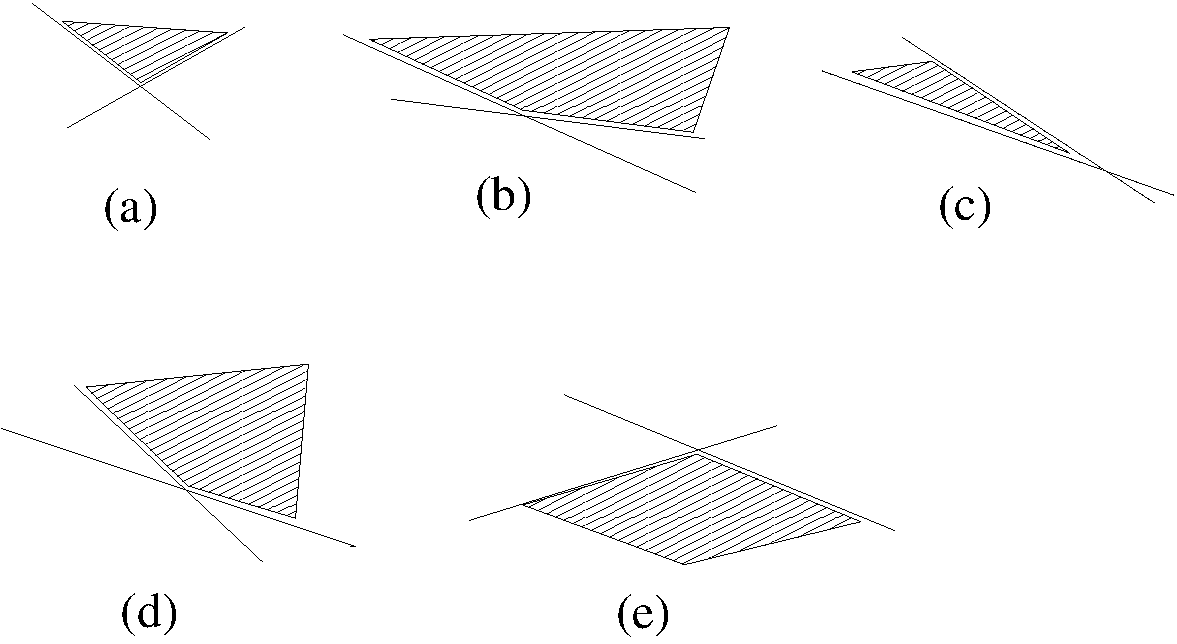
\includegraphics[width=0.8\textwidth]{Figs/Vshape.pdf}
\caption{(a) and (c) are V-shapes as the corner is optimal for the defining constraints. (b), (d), and (e) are not V-shapes since the corner is not the lowest point in the feasible region.}\label{fig:Vshapes}
\end{center}
\end{figure}

More formally, a corner is a V-shape iff the objective function vector lies in the cone of the normal vectors of the bounding hyperplanes of the constraints or equivalently if there exists $y\in \mathbb{R}^m$, $y\geq 0$ with $A^Ty=c$ \textcolor{blue}{\emph{(``This is exactly what we wrote down as the dual LP'')}}. The latter sounds rather familiar and indeed this invariant of the dual Simplex algorithm is simply the set of constraints of the dual linear program. Before we will argue that the dual Simplex algorithm is really simply the interpretation of a (primal) Simplex algorithm running on the dual linear program, let us make  the description of the dual Simplex algorithm a bit more concrete.

\begin{figure}
\begin{center}
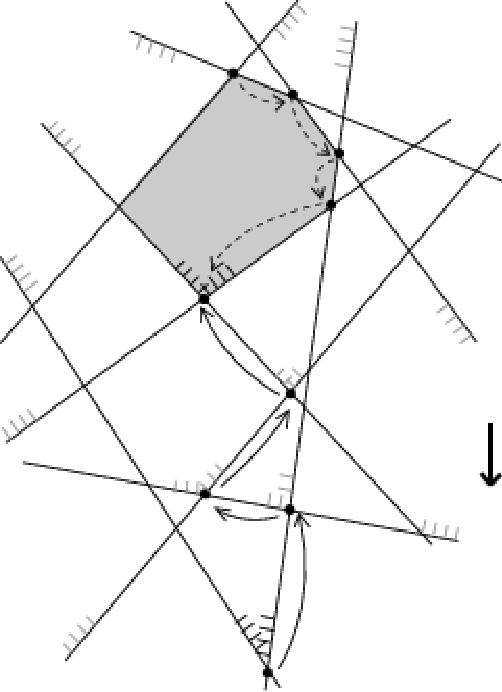
\includegraphics[width=0.5\textwidth]{Figs/PrimalDualSimplex.pdf}
\caption{Geometric Intuition of Primal (upper half \textcolor{blue}{\emph{dashed}}) and Dual Simplex (lower half \textcolor{blue}{\emph{solid}}).}\label{fig:PrimalDualSimplex}
\end{center}
\end{figure}

Consider a (primal) LP in standard form and $n$ of its constraints intersecting in a point which bound the objective function value of the LP, that is, an initial V-shape (think about how to find such an initial V-Shape).
A V-shape in the dual Simplex algorithm is a subset $B$ of $n$ constraints such that their unique intersection point $x_B$ is at the same time the optimum solution for the modified LP whose constraints are those in $B$, and the objective function is the same as that in the original LP. 
Clearly, if $x_B$ is feasible for constraints outside $B$, then $x_B$ is optimal for the whole LP.
Hence, we need to find the next V-shape only if $x_0$ violates some constraint $i \notin B$, i.e., if $a_i x_0 > b_i$.

We can easily identify a violating constraint $i$ by plugging in $x_B$ into the respective constraints. If a violating constraint $i$ is found, we use $i$ to construct the next V-shape by determining the lowest feasible point for the constraints $B\cup \{i\}$. Naively this can be done by considering all ${n\choose n-1} =n$ subsets of $B\cup\{i\}$ potential corners and use the lowest feasible one as the next \emph{V-Shap}e. Alternatively, one can consider all the intersection points of the upward rays with constraint $i$ and taking the lowest of those.
Dual Simplex continues until the V-Shape found is feasible for all other constraints (otherwise -- assuming non-degeneracy -- there is always a constraint which yields a higher V-shape). Clearly, the existence of a V-shape at some height implies that no lower feasible point exists. \emph{A V-shape whose vertex does not violate any of the other constraints is hence optimal}.

In general, note that the constraints $A^Ty=c$, $y\geq 0$ correspond to the invariant of the dual Simplex that we always have a V-shape as current solution \textcolor{blue}{\emph{(jump from V-shape to V-shape)}}, $b^Ty$ expresses the height of the current v-shape, since $y=(A_B^T)^{-1}c$ and therefore $b^Ty=b^T(A_B^T)^{-1}c=(A_B^{-1}b)^Tc = x'^T c$, where $A_B$ is the submatrix corresponding to the constraints that define the current v-shape and $x'$ the intersection point of those constraints. We have seen that max the height of the v-shape yields the same solution as aiming for the highest feasible point, and hence our dual program directly formalizes the invariants and the goal of the dual Simplex algorithm.

See Figure \ref{fig:PrimalDualSimplex} for an intuitive view on primal and dual Simplex for $n=2$.

\textcolor{blue}{\emph{``A dual simplex is basically a primal simplex on a dual LP'' }}
 
\textcolor{blue}{\emph{It is clear that the highest V-shape is the lowest point in the feasible region.}}

\paragraph{Pivoting Strategies and Degeneracies}
Termination of the dual Simplex can be argued similarly as for the primal Simplex. Since one only jumps to 'higher' V-shapes, no V-shape can be visited twice. As there are at most $m \choose n$ V-shapes, termination follows. Typically, though, there are many constraints violating the current V-shape, the choice of which constraint to consider to obtain the next V-shape strongly influences the performance of the dual Simplex algorithm in practice. Analogously to the primal Simplex, there are pivoting strategies which tend to improve the practical running times but might also run into trouble if degeneracies occur. In particular, if some constraints are \emph{orthogonal} to the objective function direction, naive pivoting rules might lead to cycling of the dual Simplex. An analogue of Bland's rule helps in that case, though.

 
\textcolor{blue}{\emph{Pivoting is a problem because there might be many violating constraints, hence there must be a strategy which one to choose.}}

\textcolor{blue}{\emph{The simplex algorithms are not known to run in polynomial time, they are very good in practice, though. Poylnomital-time Methods to solve LPs exist, e.g. Interior Point Method (in theory more practical), Ellipsoid Method.}}

\textcolor{blue}{\emph{Exam: given an LP one is to visualize and explain a primal and dual simplex algorithm.}}

\subsubsection{Interpretation of the dual Simplex algorithm as primal Simplex algorithm on the dual LP}
Let uns now convince that the dual Simplex is indeed a primal Simplex algorithm running on the dual LP but viewed in primal ($n$-dimensional) space. To that end, let us again consider a (primal) linear program (P) with $n$ variables and $m$ constraints in standard form ($m\geq n$): 	
\[
\begin{matrix}
	\max	& c_1 x_1 &+& c_2 x_2 &+& \dots &+& c_n x_n&&\\  
	\mbox{s.t.}	& a_{11} x_1 &+& a_{12} x_2&+& \dots &+&a_{1n} x_n&\leq&b_1\\
			& a_{21} x_1 &+& a_{22} x_2&+& \dots &+&a_{2n} x_n&\leq&b_2\\
			& ..	&&&&&&&&\\
			& a_{m1} x_1 &+& a_{m2} x_2&+& \dots &+&a_{mn} x_n&\leq&b_m\\
\end{matrix}
\]

According to our discussion, the following is its dual linear program (D) with $m$ variables and $n$ constraints ($m\geq n$): 

\[
\begin{matrix}
	\min& b_1 y_1 &+& b_2 y_2 &+& \dots &+& b_m y_m&&\\  
	\mbox{s.t.}	& a_{11} y_1 &+& a_{21} y_2&+& \dots &+&a_{m1} y_m&=&c_1\\
			& a_{12} y_1 &+& a_{22} y_2&+& \dots &+&a_{m2} y_m&=&c_2\\
			& ..	&&&&&&&&\\
			& a_{1n} y_1 &+& a_{2n} y_2&+& \dots &+&a_{mn} y_m&=&c_n\\
			& y_i\geq 0\\
\end{matrix}
\]

We could bring (D) again into standard form  by replacing each of the $n$ equalities by $2$ inequalities each ending up with a LP in standard form with  $2n+m$ inequalities and $m$ variables and apply the (primal) Simplex algorithm that we already know. Its geometric interpretation is taking place in $m$-dimensional space. Here a corner is always represented by $m$ linearly independent constraints fulfilled with equality. Note, though, that $n$ of these tight constraints are always formed by constraints from the set of $2n$ constraints derived from the equalities in (D). Hence, $m-n$ of the $y_j\geq 0$ constraints are also satisfied with equality, leaving only $n$ of the $y_j\geq 0$ not to be fulfilled with equality.

Focussing on these constraints in fact allows an interpretation of the Simplex algorithm run on the dual program (D) in the primal, $n$-dimensional space. The non-negative $y_j$ always select and combine as a \emph{conic combination} a set of $n$ constraints whose weighted normal vectors add up to exactly the objective function vector. In other words, the objective function vector $\overrightarrow{c}$ is always in the cone of the constraints 'selected' by non-zero $y_j$'s or in other words the selected constraints yield a lower bound for the objective function by forming a \emph{V-shape} which prevents any lower objective function value. 
With the V-shape we have associated a corner which is optimal for a subset of a constraints (at least the subset which defines the V-shape). A pivot step in the Simplex algorithm on (D) can be interpreted as identifying a constraint in the primal which is violated by the current V-shape corner and replacing one current constraint by the violating one.


\newpage

\section{LP-based Approximations of NP-hard Problems}
In this section we will discuss approximation algorithms for NP-hard problems which are based on integer linear programming formulations. Some of the methods require first the solution of a respective linear programming relaxation and then turn this possibly fractional solution into an integral solution, other methods construct primal and dual feasible solutions 'on the fly'.
 
\subsection{Running Example: The Set Cover Problem}
Consider the following problem. Given a universe $U$ of $n$ elements, a collection of subsets of $U$,
$\mathcal{S}=\{S_1, \dots, S_k\}$, and a cost function $c: \mathcal{S} \rightarrow \mathbb{R}^+$, find a minimum cost
subcollection of $\mathcal{S}' \subseteq \mathcal{S}$ that covers all elements of $U$.

\textcolor{blue}{\emph{For a general set cover it is very unlikely that a polytime Approximation-Algorithm existst that produces a solution $\mathcal{S}'$ with $c(\mathcal{S}') < log(n) * c(\mathcal{S}_{opt})$}}

In the following we will see several algorithms for this problem which both rely (at least in the analysis) on the
integer linear programming (ILP) formulation of the problem and its dual. How could we formulate the set cover problem 
as an ILP ?

\begin{eqnarray}\label{SCILP}
\mbox{min} & \displaystyle \sum_{S\in \mathcal{S}} x_S \cdot c_S\\
 u\in U: & \displaystyle \sum_{u\in S} x_S  & \geq 1 \nonumber\\
 S \in \mathcal{S}: & x_S  & \in \{0,1\}. \nonumber
\end{eqnarray}

Solving ILPs in general is quite hard, so one often considers the LP relaxation, where the integrality constraints
are dropped, here we get the following \emph{fractional covering LP}:
\begin{eqnarray}\label{SCLP}
\mbox{min} & \displaystyle \sum_{S\in \mathcal{S}} x_S \cdot c_S\\
 u\in U: & \displaystyle \sum_{u\in S} x_S  & \geq 1 \nonumber\\
 S \in \mathcal{S}: & x_S  & \geq 0\nonumber
\end{eqnarray}

Of course, this relaxation might allow better (i.e. cheaper solutions) as the integral problem, so this only yields a
\emph{lower} bound in terms of the cost of the solution. Consider the following example:
$U=\{e,f,g\}$ and $S_1=\{e,f\}$, $S_2=\{f,g\}$, $S_3=\{e,g\}$, each of unit cost. An integral cover must pick two of
the sets for a cost of $2$. But picking each set by an extent of $1/2$ yields a feasible fractional cover of cost $3/2$.

We have learned that every LP has its dual which in this case looks as follows:
\begin{eqnarray}\label{DSCLP}
\mbox{max} & \displaystyle \sum_{u\in U} y_u \\
 S\in \mathcal{S}: & \displaystyle \sum_{u\in S} y_u  & \leq c_S \nonumber\\
 u\in U: & y_u  & \geq 0\nonumber
\end{eqnarray}

This LP describes a packing problem, where the goal is to pick as many elements from the universe such that
none of a certain number of subsets is 'overpacked'.
We have seen a very similar LP before for the stable set problem, which is also a special instance
of a packing problem. In fact, set cover and packing problem are dual to
each other. Furthermore, we have learned $\sum_{u \in U} y_u \leq \sum_{S \in \mathcal{S}} x_S c_S$ for all
feasible solutions $x, y$ of the two LPs.

\subsection{Greedy Algorithm -- Dual Fitting Analysis}
The following greedy algorithm computes a cover (not necessarily optimal):
\begin{enumerate}
\item $C\leftarrow \emptyset$ \emph{($C\subseteq U$ \dots already covered elements)}
\item while $C\neq U$ do
	\begin{itemize}
	\item for each $S_i$ let $\alpha_i=\frac{\mathrm{cost}(S_i)}{|S_i-C|}$, be the cost-effectiveness of the set $S_i$
	\item let $S$ be the most cost-effective set (i.e., with minimal $a_i$ value)
	\item pick $S$ ($x_S=1$) and for each $u\in S-C$, set $\mathrm{price}(u)=\alpha$ ($y_u=\frac{\alpha}{H_n}$)
	\item $C\leftarrow C \cup S$
	\end{itemize}
\item output the picked sets
\end{enumerate}

\textcolor{blue}{\emph{
Now we want to prove that the Greedy produces a solution which is at most $\mathcal{O}(log(n))$ more costly than the optimum solution (matching the inapproximability result which states that no poly-time algorithm can approximate set cover better that logn for every instance). The Gap between the optimum integral solution to the primal problem and the solution by the Greedy algorithm is a factor of $log(n)$. Plan: see Picture from 2013-12-10 12:13
}}

\textcolor{blue}{\emph{
\begin{lemma}
The Greedy algorithm produces as solution a cover $I \subseteq \mathcal{S}$ which has cost $cost(I) \leq cost(I_{Opt}) * H_n$ where $I_{Opt} \subseteq \mathcal{S}$ is a optimum solution and $cost(X \subseteq \mathcal{S}) = \sum_{s_i \in X}{c_i}$.
\end{lemma}
}}

\textcolor{blue}{\emph{``The catch is that the dual solution is not necessarly feasible.''}}

\begin{proof}
\textcolor{blue}{\emph{The greedy algorithm computes a primal feasible integral solution of cost $\sum{X_s \cdot C_s}$.}}

\textcolor{blue}{\emph{At the same time it constructs a dual solution $y$ of exactly the same objective function value (because when primal objective function value is inceased by $c_j$, also the dual objective function value is inceased by $c_j$). This dual solution might not be feasible, though!.}}

\textcolor{blue}{\emph{The Dual constraints have the form $\forall s_i \in \mathcal{S}: \sum_{u_j \in S_i}{y_{u_j}} \leq c_j$. Consider one of these constraints, we now want to show that $\sum_{u_j \in S_i}{y_{u_j}} \leq H_n*c_i$. If so, we can determine a dual feasible solution $y' =\frac{y}{H_n}$ and $\sum{y_{u}'} = \frac{\sum{y_u}}{H_n} = \frac{\sum{x_s \cdot c_s}}{H_n}$.}}

\textcolor{blue}{\emph{We know that optimum objection function value is lower bounded by any dual feasible solution $\sum{x_{s}^{Opt} \cdot c_s} \geq \sum{y_{u}'} = \frac{\sum{y_u}}{H_n} = \frac{\sum{x_s \cdot c_s}}{H_n} \Rightarrow \sum{x_s \cdot c_s} \leq H_n * \sum{x_{s}^{Opt}} \cdot c_s$.}}

\textcolor{blue}{\emph{Now prove that for a fixed set $S \subseteq \mathcal{S}$ we have $\sum_{u \in S}{y_u} \leq H_n  \cdot c_s$. Sort the elements $u$ according to when they are covered during greedy, let that order be $u_1, u_2, \dots , u_l$ ($S = \{u_1, u_2, \dots , u_l\}$). Consider the teration of greedy when element $u_i$ was covered. Can we bound $y_{u_i}$?}}

\textcolor{blue}{\emph{In that iteation some set $S'$ was chosen for which $\frac{c_{s'}}{|s'-c|} = \alpha_{s'}$ was minimal and we set $y_{u_i} = \alpha_{s'}$.$\Rightarrow \alpha_{s'} \leq \alpha_{s}$ at that time. $\alpha_{s}= \frac{c_s}{|s-c|} \leq \frac{c_s}{l - (i+1)} \Rightarrow y_{u_i} \leq \frac{c-s}{l - (i+1)} \Rightarrow \sum_{u_i \in S}{y_{u_i}} \leq \sum_{u_i \in S}{\frac{c_s}{l - (i+1)}} = \sum_{i=1}^l{\frac{c_s}{l - (i+1)}} = c_s \cdot \sum_{i=1}^l{\frac{1}{l - (i+1)}} = \sum_{i=1}^l{\frac{1}{i}} = c_s \cdot H_l \leq c_s \cdot H_n$}}
\end{proof}

\textcolor{blue}{\emph{That analysis: 1. find primal solution, 2. derive dual feasible solution, 3. bound the gap between them. Is called dual fitting.}}

\begin{lemma}
The greedy algorithm achieves an approximation ratio of $H_n$.
\end{lemma}
\begin{proof}
We show the approximation ratio by showing that $x$ and $y$ as set by the greedy algorithm form feasible solutions
to the set cover and packing LP and $H_n \cdot \sum_{u \in U} y_u = \sum_{S \in \mathcal{S}} x_S c_S$.

Feasibility of $x$ follows from the description of the algorithm. Equally clear is that at all times 
$H_n \cdot \sum_{u \in U} y_u = \sum_{S \in \mathcal{S}} x_S c_S$ holds. So it remains to prove that
for every $S\in \mathcal{S}$, the respective packing constraint in the dual LP is satisfied.

Sort the elements of $S$ according to when they are covered during the course of the algorithm $u_1, \dots, u_l$. 
Consider the iteration when our algorithm covers element $e_i$. At this point, $S$ contains at least
$k-i+1$ uncovered elements. Therefore $S$ could cover $e_i$ at this time at an average cost of at most
$c_S/(k-i+1)$. As the algorithm always picks the most cost effective set, we get
$y_{e_i} \leq \frac{1}{H_n} \frac{c_S}{k-i+1}$. So overall we get 
\[
\sum_{i=1}^{l} y_{e_i} \leq \frac{c_S}{H_n}\cdot (\frac{1}{l}+\frac{1}{l-1}+\dots +\frac{1}{1})= \frac{H_l}{H_n}c_S\leq c_S
\]

\end{proof}



In the greedy algorithm, the (I)LP formulation was only used to proof a bound on the approximation ratio, but not part of
the algorithm. In the following we will see an approach which actually computes the solution to this LP to obtain
a set cover solution.

\noindent {\bf Remark:} In the lecture we have seen an algorithm for solving LPs in subexponential, but not polynomial time. There are
algorithms, though, which can solve linear programming problems in polynomial time (Ellipsoid and interior point methods).
So for all algorithms that follow and make use of an LP solution, we assume that it can be computed in polynomial time.
In practice though, the Simplex methods -- in spite of the superpolynomial worst-case running-time -- perform very well
and are often superior to the above guaranteed-polynomial-time methods.

\textcolor{blue}{\emph{The greedy algorithm is not LP-based, but could be analyzed via LP-ideas.}}

\textcolor{blue}{\emph{What about deterministic rounding?}}

\subsection{(Randomized) Rounding}
In the greedy algorithm, the LP relaxation was only used for the analysis, but given an optimal solution to the LP relaxation, how could we turn that into a feasible integral solution to the set cover problem, possibly with an approximation guarantee ?

\subsubsection{Simple LP rounding (Deterministic Rounding)}
The simplest strategy is to solve the  LP relaxation \ref{SCLP} of the  set cover instance to optimality and then select all sets $S$ for which $x_S>0$. This clearly ensures feasiblity, it is unclear, though, how much the objective function value might deteriorate. 
%exercise: design instances where this performs pretty badly
For the general set cover problem this strategy does not perform that well, but for special cases of set cover like for example \emph{vertex cover}, it yields reasonable approximation guarantees. In general, when the LP relaxation of an optimization problem exhibits \emph{bounded fractionality}, that is, in the optimum solution, the variables do not have arbitrary fractional values, one can often get a constant approximation.

\begin{definition}
Given a graph $G(V,E)$, the \emph{vertex cover} problem is to determine a subset $C\subseteq V$ of the nodes
such that $\forall e\in E: e\cap C\neq \emptyset$ and $|C|$ minimal.
\end{definition}

Being just a variant of the general set cover problem, a natural ILP (integer linear programming) formulation for the vertex cover problem is as follows:
\begin{eqnarray}\label{VCILP}
\mbox{min} & \displaystyle \sum_{v \in V} x_v\\
 (v,w)\in E: & x_v+x_w  & \geq 1 \nonumber\\
 v \in V: & x_v  & \in \{0,1\}. \nonumber
\end{eqnarray}
Its LP relaxation replaces $x_v \in \{0,1\}$ by the constraint $x_v\geq 0$. Assuming we have computed the optimal fractional solution to the LP relaxation, we can certainly derive a valid vertex cover by selecting all $v\in V$ with $x_v>0$. Can we prove anything about the quality of this solution? We will show in the following that in the optimal LP solution, variables only take values $0,\frac{1}{2},1$, hence our simple rounding scheme yields a solution of cost at most twice the cost of the LP relaxation (since in the worst case, a variable doubles its value) and therefore is also a $2$-approximation to the vertex cover problem.

\begin{lemma}
In the LP relaxation of the vertex cover problem, variables only take values $0,\frac{1}{2},1$ in the optimum solution.
\end{lemma}
\begin{proof}
We show even a stronger statement, namely that every corner of the polyhedron defined above only takes values $0,\frac{1}{2},1$ -- we also say, that all corners are \emph{half-integral}. Let $x$ be a feasible solution which 
is not half-integral. By showing that $x$ can be expressed as the convex combination of two feasible solutions, it is clear that $x$ cannot be a corner.

Consider all $v\in V$ for which $x_v\notin \{0,\frac{1}{2}, 1\}$, and let
\[
	V_+=\{v|\frac{1}{2}<x_v<1\},\quad V_-=\{v|0<x_v<\frac{1}{2}\}
\]
For some $\epsilon>0$ define solutions $y$ and $z$ as follows:
\[
	y_v= \left\{ \begin{array}{rl} x_v+\epsilon& v\in V_+\\ x_v-\epsilon& v\in V_-\\ x_v& otherwise \end{array} \right., \quad z_v= \left\{ \begin{array}{rl} x_v-\epsilon& v\in V_+\\ x_v+\epsilon& v\in V_-\\ x_v& otherwise \end{array} \right.
\]
As $V_+\cap V_-=\emptyset$, we know that $x, y, z$ are all distinct, and clearly $x=\frac{1}{2}(y+z)$. It remains to show that $y$ and $z$ are indeed feasible. Consider one particular edge constraint and the case that $x_v+x_w>1$. Clearly, a small enough choice of $\epsilon$ keeps this constraint satisfied. On the other hand, if $x_v+x_w=1$, either $x_v=x_w=\frac{1}{2}$, or $v\in V_+, w\in V_-$ or vice versa. In all cases, the modified solutions $y$ and $z$ still satisfy this constraint with equality. 
\end{proof}
In general, if we can prove for an LP relaxation \emph{bounded fractionality}, it is often possible to derive an integral solution with some approximation guarantee.

\subsubsection{Frequency-based LP rounding}
In the following denote by $f$ the maximal number of occurrences of an element $u\in U$ in the sets $S_1,\dots, S_k$, i.e.
$f=\max_{u\in U} |\{S_i: u\in S_i\}|$. We consider the following simple algorithm:
\begin{enumerate}
\item Find an optimal solution to the LP relaxation of the set cover problem
\item Pick all sets $S$ for which $x_S\geq 1/f$
\end{enumerate}

\textcolor{blue}{\emph{\emph{Observation 1:} Objective function value (compared to the LP-solution) increases by at most a factor of $f$}}

\textcolor{blue}{\emph{\emph{Observation 2:} Each constant for a $u\in U \sum_{S_i{x_i \geq 1}}$. The left hand-side consists of at most $f$ terms. Assume all $x_i < 1/f$ (which would yield an infeasible solution), then the sum on the left is $ < f \cdot 1/f = 1$. $\Rightarrow$ at least one $x_i \geq 1/f$ which is then rounded up to 1 $\Rightarrow$ rounded-up solution is feasible.}}

\begin{lemma}
The simple $1/f$ LP-rounding algorithm achieves an approximation factor of $f$.
\end{lemma}
\begin{proof}
Let $\mathcal{C}$ be the collection of picked sets. Consider an arbitrary element $u$. Since $u$ is in at most $f$ sets,
at least on of the respective sets must be picked to an amount of $\geq 1/f$. Hence $\mathcal{C}$ is a valid cover.
On the other hand, the value of each $x_S$ is increased by at most a factor of $f$, so the overall objective function value
increases by at most a factor of $f$.
\end{proof}

It happens that the set cover instance derived from the vertex cover problem has an $f$-value of $2$, since any $u\in U$ (edge) appears in exactly two 'sets', namely the sets corresponding to the endpoints of the edge. Hence, in this way we can also obtain a $2$-approximation to the set cover problem.
% exercise: find instance of set cover where this approach yields horrible approximation


\subsubsection{Randomized LP rounding for the Set Cover problem}
A more sophisticated way to turn the LP solution into a feasible integral solution is to interpret the LP values
as probabilities and flip coins accordingly.

Let $x^*=p$ be the optimal solution to the LP relaxation of the set cover problem, $\mathrm{OPT}_{LP}$ its objective function value.
For each set $S$ we pick it with probability $x^*_S=p_S$ into $\mathcal{C}$. What is the expected cost of $\mathcal{C}$ ? 
\textcolor{blue}{\emph{ Let $x^*$ be the rounded values.}}

\[
	{\bf E}[\mathrm{cost}(\mathcal{C})]=\sum_{S\in \mathcal{S}} p_S\cdot c_S=\mathrm{OPT}_{LP}
\]

The collection $\mathcal{C}$ not necessarily covers $U$, but let us look at the probability by which an element $u\in U$ is covered.
Assume $u$ appears in $l$ sets $S_1, \dots, S_l$. As $u$ is fractionally covered, we have $p_1+p_2+\dots +p_l\geq 1$.

\textcolor{blue}{\emph{$u$ is not covered if and only if $S_1$ was not picked, $S_2$ was not picket $\cdots S_l$ was not picked. A set $S_i$ was not picked with probability $(1-x^*)$. $u$ was not covered/one of the sets were picked with the propability $\Pi_{i=1}^l(1-x_i^*)$}}

As the probability for $u$ being covered is minimized if $p_i=1/l$, we get the following bound:
\[
	{\bf \mathrm{Pr}}(a \mathrm{~ covered~by~ }\mathcal{C}) \geq 1 - (1-\frac{1}{l})^l \geq 1- \frac{1}{e}
\]

The last inequality follows from $(1+\frac{1}{n})^n < e < (1+\frac{1}{n})^{n+1}$ since
$e<(\frac{n+1}{n})^{n+1} \Leftrightarrow (\frac{n}{n+1})^{n+1} < 1/e \Leftrightarrow (\frac{n+1}{n+1}-\frac{1}{n+1})^{n+1}<1/e$.
This means, each element from $u$ is covered with a constant probability.

\textcolor{blue}{\emph{Look at the following experiment: We flip a fair coin until getting heads. With probability $\frac{1}{2}$ we succeed in the first flip. With the probability $\frac{1}{2} \cdot \frac{1}{2}$ we succeed in the second flip $\cdots \Rightarrow$ expected number of coinflips until heads appears is $\sum_{i = 1}^\infty{ i \cdot Pr(we~succeed~in~step~i)} = \sum_{i = 1}^\infty{ i \cdot (\frac{1}{2})^i} \rightarrow 2$. also see Coupon-Collector-Problem}}

To obtain a valid set cover, independently pick $c \log n$ such subcollections and compute their union, say $\mathcal{C}'$, where $c$
is a constant such that
\[
	(\frac{1}{e})^{c\log n }\leq \frac{1}{4n}
\]
at this point we have ${\bf \mathrm{Pr}}(\mathrm{a~not~covered~by~}\mathcal{C}') \leq \frac{1}{e}^{c\log n} \leq \frac{1}{4n}$
\textcolor{blue}{\emph{(after $c\cdot \log n$ iterations)}}and summing over all $u\in U$ we get:
\[
	{\bf \mathrm{Pr}}(\mathcal{C}'\mathrm{~not~a~valid~set~cover}) \leq n\cdot \frac{1}{4n}=\frac{1}{4}
\]
For the cost of the obtained solution we get 
\[
	{\bf E}[\mathrm{cost}(\mathcal{C})']\leq c\cdot \log n\cdot \mathrm{OPT}_{LP}
\]

Applying Markov's inequality ($\mathrm{Pr}(X\geq t)\leq \frac{E(X)}{t}$)
with $t=\mathrm{OPT}_{LP}\cdot 4c \log n$ we get
\[
	{\bf \mathrm{Pr}}[\mathrm{cost}(\mathcal{C})'\geq 4\cdot c \log n \cdot \mathrm{OPT}_{LP}]\leq \frac{1}{4} 
\]
So the union of the two bad events happens with probability at most $1/2$, and therefore 
\[
	{\bf \mathrm{Pr}}(\mathcal{C}'\mathrm{~a~valid~set~cover~with~cost~}\leq 4\cdot c \log n \cdot \mathrm{OPT}_{LP}) 
		\geq \frac{1}{2}
\]

We can verify in polynomial time whether $\mathcal{C}'$ satisfies both conditions and repeat if not. The expected number of
repetitions needed until we succeed is at most $2$.


\subsection{The Primal-Dual Scheme}
The last paradigm for designing approximation algorithms based on linear programming is the \emph{Primal-Dual Scheme}. The high-level idea of the primal dual scheme is to start with a pair of solutions $(x_0, y_0)$ where $x_0$ is a primal infeasible solution and $y_0$ a dual \emph{feasible} solution, and then start increasing dual variables and hence the objective function of the dual solution while maintaining dual feasibility. During that process, dual constraints become tight which is regarded as a guidance for which primal variable to increase.

Again let us consider the LP relaxiation of the set cover ILP and its dual:

\begin{minipage}{0.5\textwidth}
\begin{eqnarray}
\mbox{min} & \displaystyle \sum_{S\in \mathcal{S}} x_S \cdot c_S \nonumber \\
 \forall u\in U: & \displaystyle \sum_{u\in S} x_S  & \geq 1 \nonumber\\
 \forall S \in \mathcal{S}: & x_S  & \geq 0. \nonumber
\end{eqnarray}
\end{minipage}
\begin{minipage}{0.5\textwidth}
\begin{eqnarray}
\mbox{max} & \displaystyle \sum_{u\in U} y_u \nonumber \\
\forall S\in \mathcal{S}: & \displaystyle \sum_{u\in S} y_u  & \leq c_S \nonumber\\
\forall u\in U: & y_u  & \geq 0\nonumber
\end{eqnarray}
\end{minipage}
\\[.5cm]

\textcolor{blue}{\emph{\emph{Complementary Slackness Condition:} Let ($x^*, y^*$) be optimal solutions to primal ($x^*$) and dual ($y^*$) LP. Then we have:
\begin{itemize}
	\item if $x_i^* > 0 \Rightarrow$ Corresponding constraint in the dual is tight for $y^*$.
	\item if $y_j^* > 0 \Rightarrow$ Corresponding contraint in the primal is tight for $x^*$.
\end{itemize}
``Look up how the dual is derived''
}}
\ \\

The algorithm works as follows:
\begin{enumerate}
\item Start with a primal solution $x=0$ and a dual (feasible) solution $y=0$
\item Pick some uncovered element $u\in U$ and increase its dual variable $y_u$ until dual
		constraints becomes tight; add the respective sets ($x_S=1$) to our cover $C$. \textcolor{blue}{\emph{stop increasing $y_u$ and pick all sets $S \in \mathcal{S}$ whose corresponding constraint in the dual become tight (means the left hand side is equal the right hand side).}}
\item if there are still uncovered elements, go to 2., otherwise ouput the cover $C$
\end{enumerate}

\textcolor{blue}{\emph{Example: (picture from 2014-01-16)
Red = setcover from Greedy. Blue = optimal. If the variable in set 5 is increased then the constraint corresponding to set 5 becomes tight. Which means that set 5 and 1 is picked. doing it again with another variable, then we would pick 4 sets. which would not necessarily be better than the greedy algorithm.\\Clearly the algorithm produces a feasible cover (otherwise some $y_u$ would be increased); dual solution remains feasible all the time since we stop increasing once dual constraint gets tight.\\ $\Rightarrow$ the algorithm terminates with feasible solution $\widetilde{x}, \widetilde{y}$ (which both are integral) and we need to analyze the ration $\frac{c^T \widetilde{x}}{1^T \widetilde{y}}$.}}

\ \\

First observe that\begin{eqnarray}\label{SCILP}
\mbox{min} & \displaystyle \sum_{S\in \mathcal{S}} x_S \cdot c_S\\
 u\in U: & \displaystyle \sum_{u\in S} x_S  & \geq 1 \nonumber\\
 S \in \mathcal{S}: & x_S  & \in \{0,1\}. \nonumber
\end{eqnarray} the algorithm clearly produces a valid cover as if there was an uncovered element after termination, the algorithm would have increased its dual variable until some set constraint would have become tight (such a constraint must exist as $u\in U$ must be in some set). Furthermore, the dual solution remains feasible all the time. Hence the algorithm terminates with feasible solutions $\widetilde{x}$, $\widetilde{y}$ and we are interested in the ratio $\frac{\widetilde{x}}{\widetilde{y}}$. In the ideal case, this ratio is $1$ which would imply that we have found an optimum solution.


\begin{lemma}
Let $f$ be the maximum frequency of an element $u\in U$ in the sets. Then we have 
$c^T\widetilde{x}\leq f 1^T\widetilde{y}$.
\end{lemma}
\begin{proof}
We have
\[
	c^T\widetilde{x} = \sum_{S\in C} c_S = \sum_{S\in C} \sum_{u\in S} y_u \leq f \cdot \sum_{u\in U} y_u = f \cdot 1^T \widetilde{y}
\]
since we have picked set $S$ when the respective dual constraint became tight \textcolor{blue}{\emph{(which means $\sum_{u \in S}{y_u} = c_S$)}}. In the resulting double sum we count each $y_u$ at most as often as it appears in some set (hence at most $f$ times).
\end{proof}

As an example consider the worst-case instance for the greedy set cover algorithm and try to follow the primal dual algorithm.

\subsection{Further Example: Uncapacitated Facility Location}

\textcolor{blue}{\emph{siehe Aufschrieb...}}

The uncapacitated facility location problem can be stated as follows, we are given:
\begin{itemize}
\item a set of locations $V$ with associated distance measure $c_{ij}$ between the locations which satisfies the triangle inequality
\item a subset $F\subset V$ of potential facility locations, each potential location $i\in F$ associated with an opening cost $f_i\geq 0$
\item demand locations/clients $D=V-F$; connecting a location $j\in D$ with a facility opened at $i\in F$ incurs connection cost $c_{ij}$ 
\end{itemize}

The goal is to determine a subset $F'\subseteq F$ of locations where to open facilities and assign each demand location $j\in D$ to its nearest open facility, such that the total cost (comprising opening and connection costs)
\[
	\sum_{i\in F'} f_i + \sum_{j\in D} \min_{i\in F'} c_{ij}
\] 
is minimized.

This problem at first sights seems rather difficult since optimizing only for one objective -- e.g. opening only few facilities -- has a negative effect on the other objective -- the connection costs will become larger. And vice versa, aiming for low connection costs typically requires opening many facilities -- which increases the opening costs.

We start with an integer linear programming formulation introducing binary variables $y_i$ to decide which facilities to open (=1) and variables $x_{ij}$ to decide to which facility a demand location is connected to, more precisely $x_{ij}=1$ if client $j\in D$ is connected to the (openend) facility $i\in F$.


\begin{eqnarray}\label{UFL}
\mbox{min} & \displaystyle \sum_{i\in F}{y_i f_i} + \sum_{j\in D}{\sum_{i\in F}{x_{ij}c_{ij}}}\\
 \forall j\in D: & \sum_{i\in F} x_{ij}  & = 1 \nonumber\\
 \forall i\in F, \forall j\in D: & y_i &\geq x_{ij} \nonumber\\
 & y_i, x_{ij}&\in \{0,1\} \nonumber
\end{eqnarray}

Here, the first constraint enforces that every client is connected to some facility, the second constraint makes sure that a facility is openend if some client is connected to it. The LP relaxation naturally arises by replacing the integrality constraints on $y_i, x_{ij}$ by respective $\geq 0$ constraints.

The primal of the LP relaxation looks as follows:
\begin{eqnarray}\label{UFLP}
\mbox{min} & \displaystyle \sum_{i\in F}{y_i f_i} + \sum_{j\in D}{\sum_{i\in F}{x_{ij}c_{ij}}}\\
 \forall j\in D: & \sum_{i\in F} x_{ij}  & = 1 \nonumber\\
 \forall i\in F, \forall j\in D: & y_i &\geq x_{ij} \nonumber\\
 & y_i, x_{ij}&\geq 0 \nonumber
\end{eqnarray}

The dual of the LP relaxation looks as follows:
\begin{eqnarray}\label{UFLD}
\mbox{max} & \displaystyle \sum v_j \\
 \forall i\in F: & \sum_{j\in D} w_{ij}  & \leq f_i \nonumber\\
 \forall i\in F, \forall j\in D: & v_j - w_{ij} &\leq c_{ij} \nonumber\\
 \forall i\in F, \forall j\in D: & w_{ij}&\geq 0 \nonumber
\end{eqnarray}

Let us first start with a small Lemma exhibiting some property of primal and dual optimal solutions.

\begin{lemma}
Let $(x^*, y^*)$ be an optimal solution to the primal LP, $(v^*, w^*)$ an optimal solution to the dual LP. Then $x_{ij}>0$ implies $c_{ij}\leq v_j^*$.
\end{lemma}
\begin{proof}
Due to complementary slackness we know: $x^*_{ij}>0$ implies $c_{ij}=v^*_j-w_{ij}$ and together with $w_{ij}\geq 0$ yields the lemma.
\end{proof}

\begin{definition}
For a LP-solution $x^*$ we say that $i\in F$ \emph{neighbors} $j\in D$ if $x^*_{ij}>0$ (and equally $j\in D$ \emph{neighbors} $i\in F$).
\end{definition}

Based on that definition we define the following neighborhoods of a client $j\in D$:
\[
	N(j):=\{i\in F: i\mbox{ neighbors } j\} 
\]
and
\[
	N^2(j):=\{k\in D: k\mbox{ neighbors some } i\in N(j)\} = \{k\in D: \exists i \in F: i \in N(j) \mbox{ and } i \in N(k)\} = \mbox{ 2-hop-neighbor }
\]

\subsubsection{Deterministic Rounding}
\textcolor{blue}{\emph{This yields a 4-Approximation.}}
Let us start with a simple rounding scheme which turns a fractional LP solution into a not too expensive integral solution.
\begin{enumerate}
\item compute optimal solutions $(x^*, y^*)$ and $(v^*,w^*)$ to primal and dual LP
\item $S\leftarrow D$
\item $F'\leftarrow\emptyset$
\item while $S\neq \emptyset$
	\begin{enumerate}
	\item choose $j\in S$ with $v_j^*$ minimal
	\item pick $i\in N(j)$ with $f_i$ minimal and open $i$, i.e. $F' \leftarrow F' \cup \{i\}$ 
	\item assign $j$ and all unassigned clients $k \in N^2(j)$ to $i$  \textcolor{blue}{\emph{(also in the two-hop-neighborhood, this is fulfills the triangle inequality.)}}
	\item $S\leftarrow S-\{j\}-N^2(j)$
	\end{enumerate}
\end{enumerate}

Let us now prove that this algorithms yields a solution which is at most a factor of $4$ away from the optimum. This result is due to Shmoys/Tardos/Aardal'97 and Chudak'98.

\begin{theorem}
The above algorithm produces a solution of cost at most $4$ times the optimum solution.
\end{theorem}
\begin{proof}
Consider an iteration where $j\in S\subset D$ and $i\in N(j)\subset F$ were picked as described. Then we have:
\[
	f_i=f_i\cdot \sum_{k\in N(j)}x^*_{kj}= \sum_{k\in N(j)}f_i x^*_{kj} \leq \sum_{k\in N(j)}f_k x^*_{kj}\leq \sum_{k\in N(j)} f_k y^*_k
\]
Here the first equality holds since $\sum_{k\in N(j)}x^*_{kj}=1$, the first inequality holds since we have picked the cheapest $i\in N(j)$, and the second inequality holds by definition. To bound the total opening cost we would like to have that
\[
	\sum_{i\in F'} f_i \leq \sum_{i\in F}f_iy_i^* \leq OPT_{Prinal}
\]
The facility opening costs are always charged to a neighborhood (consisting of facilities) of a single client. Since then all the neighbors (clients) of this neighborhood are removed from $S$, none of the facilities in $N(j)$ can be charged again. Hence, the total opening costs are clearly bounded by the objective function value of the LP optimum.

It remains to bound the connection costs. According to our previous Lemma, we know that the cost of connecting $j$ to $i$ is $c_{ij}\leq v^*_j$. The connection costs for the elements $k\in N^2(j)$ which have a common neighbor $l$ with $i$ are
\[
	c_{ik}\leq c_{lk}+ c_{lj} + c_{ij} \leq v^*_j+v^*_j+v^*_k\leq 3 v^*_k
\]
where the latter inequality follows from the fact that we chose $j\in S$ with $v^*_j$ minimal.

So the total cost can be bounded by:
\[
	\sum_{i\in F} f_iy^*_i + 3\sum_{j\in D}v^*_j \leq OPT_{primal}+ 3 OPT_{dual}=4 OPT_{primal}\leq 4 OPT_{int}
\]
\end{proof}

\subsubsection{(Slightly) Randomized Rounding}
Let us now try to improve the approximation factor by devising a \emph{randomized} rounding procedure. To that end, we define
\[
	C^*_j:=\sum_{i\in F}c_{ij}x^*_{ij}
\]

and rephrase the selection rules for $j\in S$ and $i\in N(j)$ as follows:
\begin{enumerate}
\item compute optimal solutions $(x^*, y^*)$ and $(v^*,w^*)$ to primal and dual LP
\item $S\leftarrow D$ \textcolor{blue}{\emph{(S = the clients that have not been served yet.)}}
\item $F'\leftarrow\emptyset$
\item while $S\neq \emptyset$
	\begin{enumerate}
	\item choose $j\in S$ with $(v_j^*+C_j^*)$ minimal
	\item choose $i\in N(j)$ randomly according to the probability distribution given by $x^*_{ij}$ and open $i$
	\item assign $j$ and all unassigned clients in $N^2(j)$ to $i$
	\item $S\leftarrow S-\{j\}-N^2(j)$
	\end{enumerate}
\end{enumerate}

We can now prove the following stronger statement about the approximation quality of this modified algorithm:

\begin{theorem}
The above randomized rounding algorithm yields a solution with expected objective function value at most $3$ times the optimum.
\end{theorem}
\begin{proof}
Again, we consider an iteration where some $j\in S$ was picked. Let $F$ be a random variable denoting the facility opening cost in this round. Clearly the expected value of $F$ is
\[
E(F)=\sum_{i\in N(j)}f_i x^*_{ij}\leq \sum_{i\in N(j)} f_i y^*_i
\]

\textcolor{blue}{\emph{($\sum_{i\in N(j)}$ = Sum over neighborhood)}}

Now let $A_k$ be a random variable denoting the assignment cost of client $k$ to facility $i$. The expected assignment cost of $j$ to $i$ is
\[
	E(A_j)=\sum_{i\in N(j)} c_{ij} x^*_{ij}=C_j^*
\] 
The expected assignment cost for a $k\in N^2(j)$, $k\neq j$ where $k\in D$ neighbors $l\in F$ which neighbors $j\in D$ is \textcolor{blue}{\emph{(using triangle inequality. See Picture from 2014-01-28. Lemma 14)}}
\[
	E(A_k)\leq c_{lk} + c_{lj} + \sum_{i\in N(j)}c_{ij}x^*_{ij}\leq v^*_k + v^*_j+ C^*_j \leq v^*_k + v^*_k + C^*_k=2v^*_k +C^*_k
\]
where the last inequality follows from the choice of $j\in S$.

So the total cost can be bounded as follows:
\[
	\sum_{i\in F} f_i y^*_i + \sum_{j\in D} (2v_j^* + C^*_j) = \sum_{i\in F}f_i y^*_i + \sum_{j\in D}C^*_j +  2\sum_{j\in D} v^*_j=OPT_{LP}+2 OPT_{DLP}\leq 3 OPT_{int}
\]

\end{proof}

\textcolor{blue}{\emph{This is not the 'natural' randomized rounding algorithm.}}

A variant of the 'natural' randomized Rounding algorithm where one randomly chooses facilities to Open according to the probability $y_i^*$ and then connect each client to its closest open facility can be proven to be a 1.736 Approximation.

It can be shown that no poly-time algorihtm can approximate both than 1.627, unless P = NP

\subsubsection{Primal-Dual Algorithm}

\begin{definition}
For a LP-solution $x^*$ we say that $i \in F$ neighbors $j \in D$ if $v_j^* \geq c_{ij}$ (and equaly $j \in D$ neighbors $i \in F$).
\end{definition}

Neighborhoods $N(j)$, $N^2(j)$ are defined as before.

\begin{enumerate}
\item $v \leftarrow 0$, $w \leftarrow 0$
\item $A \leftarrow 0$
\item $l \leftarrow 0$
\item $S \leftarrow D$
\item while $S \neq 0$
\begin{enumerate}
	\item $l \leftarrow l + 1$
	\item increase $v_j$ for all $j \in S$ and all $w_{ij}$ for all $i\in N(j)$, $j \in S$ uniformly until $\exists i_l \in F: \sum_{j\in D}{w_{ij} = f_i}$
	\item $A \leftarrow A \cup \{i_l\}$
	\item $S \leftarrow S - N(i_l)$
\end{enumerate}
\end{enumerate}

Algorithm obviously produces feasible solution in primal and dual.

For the facility opening costs we observe:
\[
	\sum_{i\in A}{f_i} = \sum_{i\in A}{\sum_{j \in D}{w_{ij}}} = \sum_{i\in A}{\sum_{j \in D}{\max(v_j - c_{ij}, 0)}} = \sum_{j\in D}{\sum_{c \in N(j) \cap A}{(v_j-c_{ij})}}
\]

\textcolor{blue}{\emph{Sum up over all client and their neighborhood. Problem there could be more than one open facility in the neigborhood, which makes it dificult.}}

If we had $|N(j) \cap A| = 1 \forall j \in D$ with $i(j)$ being the unique open facility in the neighborhood of $j$, we could continue 
\[
	= \sum_{j \in D}{(v_j - c_{i(j)j}) \leq \sum_{j \in D}{v_j} \leq OPT}
\]

Unfortunately that's not true for $A$, but we can prune $A$ to $A'$ with this property without incuring too high additonal connection costs: \textcolor{blue}{\emph{see second Picture from 2014-01-28}}

\begin{enumerate}
	\item $A' \leftarrow A$
	\item for $k = 1$ to $l$
		\begin{enumerate}
			\item if $i_k \in A$ open $i_k$, $A' \leftarrow A' - N^2(i_k)$ and assign unassigned $j \in N(i_k) \cup N^3(i_k)$ to $i_k$ 
		\end{enumerate}
\end{enumerate}

$A'$ denote the resulting set of facilities to open.

\begin{lemma}
	$\forall j \in D: |A' \cap N(j)| \leq 1$
\end{lemma}

\begin{proof}
Assume otherwise, i.e. $i_a$, $i_b \in A' \cap N(j)$, $ a < b$. Then $i_b$ should have been removed from $A'$ when $i_a$ was considered. 
\end{proof}

Now there are some $j \in D$ wiht $N(j) \cap A' = 0$. We claim that their connection cost is not too big, i.e. $c_{i(j)j} \leq 3 v_j$.
As for such $j$ all facilities $i \in N(j) \cap A$ have ... indices than $i(j)$, hence $v_j \geq v_k \forall k \in N(i(j))$. Assume $j$ neighbors $i$ neighbors $k$ neighbors $i(j)$

\textcolor{blue}{\emph{see third picture from 2014-01-28}}

\textcolor{blue}{\emph{see fourth picture from 2014-01-28 ff}}



\end{document}